\documentclass[letterpaper,10pt]{book}
% Change to 10 pt
\usepackage{pdfpages}
\usepackage{morewrites}			% to counteract the no write space problem
\setcounter{tocdepth}{6}

\usepackage[framemethod=TikZ]{mdframed}

\usepackage{fancyhdr}

\usepackage{paralist}
\usepackage{amsmath}
\usepackage{amsfonts}
\usepackage{amssymb}
\usepackage{graphicx}

\usepackage{datetime}
%\usepackage{ulem}

%\usepackage[nottoc]{toobibind}

\usepackage[inline]{enumitem}

% Outer margin at 2.50 is exacty correct to fit the ``corruption alert'' tables
\usepackage[inner=1.0in, outer=2.50in, top=2.54cm,bottom=2.54cm, marginparwidth=2.25in]{geometry}

\usepackage{marginnote}
\usepackage{longtable}
\usepackage{booktabs}
\usepackage{xcolor}

\usepackage{soul}

%%%%%%%%%%%%
\definecolor{ForestGreen}{rgb}{0.00,0.29,0.098}
%%%%%%%%%%%%

\usepackage{marginnote}

\usepackage{imakeidx} 
\usepackage[
	backref=true,
	style=numeric,
%	citestyle=numeric,
	backend=bibtex
	]{biblatex}
\usepackage[driverfallback=hypertex,colorlinks=True]{hyperref}
\usepackage{cleveref}

\makeindex[name=scripture,columnsep=20pt, columnseprule=True,columns=3, title=Scripture References]
\makeindex[name=speaker,columnsep=20pt, columnseprule=True,,columns=2, title=Sermon Creator]
\makeindex[name=series,columnsep=20pt, columnseprule=True,,columns=2, title=Sermon Series]
\makeindex[name=date,columnsep=20pt, columnseprule=True,columns=2, title=Sermon Date]
\makeindex[name=event,columnsep=20pt, columnseprule=True,columns=2, title=Event]
\makeindex[name=topic,columnsep=20pt, columnseprule=True,columns=2, title=Topic]
\makeindex[name=AWIP,columnsep=20pt, columnseprule=True,columns=3, title=All Words in Passage]
\makeindex[name=NWIV,columnsep=20pt, columnseprule=True,columns=3, title=Number of Words in Verse]
\makeindex[name=PNIP,columnsep=20pt, columnseprule=True,columns=3, title=Proper Names in Passage]
\makeindex[name=PEIP,columnsep=20pt, columnseprule=True,columns=2, title=Prophetic Events in Passage]
\makeindex[name=TWPAQ,columnsep=20pt, columnseprule=True,columns=1, title=13-Word Phrases and Quotes]
\makeindex[name=PFTTIS,columnsep=20pt, columnseprule=False,columns=3, title=Phrases found 13 times in scripture]
\makeindex[name=WFTTIS,columnsep=20pt, columnseprule=False,columns=3, title=Words found 13 times in scripture]
\makeindex[name=WFITV,columnsep=20pt, columnseprule=False,columns=3, title=Words found in exactly 13 verses]
\makeindex[name=EVENTS,columnsep=20pt, columnseprule=False,columns=2, title=Sermon Log by Place]
\makeindex[name=QUESTIONS,columnsep=20pt, columnseprule=False,columns=2, title=Bible Questions]
\makeindex[name=DOCTRINES,columnsep=20pt, columnseprule=False,columns=2, title=Doctrines]
\makeindex[name=SONGS,columnsep=20pt, columnseprule=False,columns=1, title=Songs]
\makeindex[name=LOCATION,columnsep=20pt, columnseprule=False,columns= 2, title=Location]
\makeindex[name=FACEBOOK,columnsep=20pt, columnseprule=False,columns=2, title=Facebook]
\makeindex[name=DEVOTIONAL,columnsep=20pt, columnseprule=False,columns=2, title=Devotional Items]
%%%%%%%%%%%%%%%%% EXTRA COLORS
\definecolor{champagne}{rgb}{0.97,0.91,0.81}
\definecolor{bone}{rgb}{0.89,0.85,0.79}
\pagestyle{fancy}
\fancyhf{}
\fancyhead[LE,RO]{\today}
\fancyhead[RE,LO]{Daily Bible Reading}
\fancyhead[CE,CO]{-page \thepage  - }

\fancyfoot[CO,CE]{\leftmark}
%\fancyfoot[LE,RO]{CSCE 692, HW1}

\title{DBR\\
Daily \\ Reads}
\author{Keith Anthony \\
\today }
%+/ffffff +   \pagenumbering{gobble}
\bibliography{Bibliographies/All20220122}

\setlength{\fboxsep}{1.0pt}

\usepackage[utf8]{inputenc}
\usepackage{tikz}

\begin{document}
%%%%%%%%%%%% Tile Page

\begin{titlepage}

\begin{flushright}
\rightskip=-2.5cm
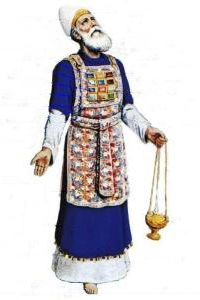
\includegraphics[width=50mm,scale=1.5]{Extras/Melchisedec.jpg}
\vspace{0.4in}  % Create a title for the document and write it in bold font
\LARGE{\textbf{\date}} % Again, do a line break
\linebreak 
% Create a subtitle \large{with Outlines, Statistics, Cross References, and Notes}
\vspace{0.5in}
\begin{flushleft}
\LARGE{Day \#67: Tuesday, 8 March 2022  PLAIN \\}\vspace{0.25in}
\LARGE{Joshua 7-9 Psalm 67 Proverb 8}
\end{flushleft}
\vspace{0.6in}
\bigskip

\normalsize{Xenia, Oh.\\}
\normalsize{created: \today}
\vspace{1.3in}

\end{flushright}
\end{titlepage}

\newpage 
\tableofcontents\hypertarget{TOC}{}
\listoffigures
\listoftables

\hyphenation{A-bim-e-lech bre-thren E-phra-im  Gib-e-o-nites Jer-u-sa-lem through-out Phil-i-stines The-o-phil-us Am-a-le-kites ven-geance Mesh-el-e-mi-ah onan-ism Phar-a-oh thoughts grev-ous-ness Hach-a-liah adul-ter-er Shad-rach}

%%%%%%%%%%%%%%%%% EXTRA COLORS
%%%%%%%%%%%%%%%%% EXTRA COLORS
%%%%%%%%%%%%%%%%% EXTRA COLORS
\definecolor{champagne}{rgb}{0.97,0.91,0.81}
\definecolor{bone}{rgb}{0.89,0.85,0.79}

\definecolor{ForestGreen}{rgb}{0.00,0.29,0.098}
\definecolor{GIVING}{cmyk}{1,0.0,0.72,.1}

\definecolor{MLPE}{cmyk}{1,1,0,.45}
\definecolor{SOCCER}{cmyk}{.77, 0, .42, .49}
\definecolor{PAYBILL}{cmyk}{0,0.83,0.76,0.07}
\definecolor{SERMON}{cmyk}{.14,.9,0,.30} % aka seance \href{http://www.flatuicolorpicker.com/purple-cmyk-color-model/}{seance}
\definecolor{BIBLE}{cmyk}{0,.17,.74,.17}
\definecolor{WORKBLUE}{cmyk}{1, .5, 0, .6}
\definecolor{myOrange}{cmyk}{0, .4, .98, .03}
\definecolor{myTan}{cmyk}{0.0,.07,.17,.10}
\definecolor{myRed}{cmyk}{0,1,1,0}
\definecolor{myWhite}{cmyk}{0,0,0,0}
\definecolor{BLUESoD}{cmyk}{.97,.84,0,.04}
\definecolor{WHITE}{cmyk}{0,0,0,0}
\definecolor{OLDGOLD}{cmyk}{0.05,0.3,1.00,0}
\definecolor{CASTLETON}{cmyk}{1,0,0.31,0.66}
\definecolor{cadmiumgreen}{rgb}{0.0, 0.42, 0.24}
\definecolor{jungle}{rgb}{0.203,0.4882,0.1718}
\definecolor{MYGOLD}{rgb}{1,.84,0}

\definecolor{MYLIGHTGRAY}{rgb}{.85,.85,.85}

\definecolor{codegreen}{rgb}{0,0.6,0}
\definecolor{codegray}{rgb}{0.5,0.5,0.5}
\definecolor{codepurple}{rgb}{0.58,0,0.82}
\definecolor{backcolour}{rgb}{0.95,0.95,0.92}


\mdfdefinestyle{MyFrame}{%
    linecolor=blue,
    outerlinewidth=2pt,
    roundcorner=5pt,
    innertopmargin=\baselineskip,
    innerbottommargin=\baselineskip,
    innerrightmargin=10pt,
    innerleftmargin=10pt,
    backgroundcolor=gray!25!white}


\mdfdefinestyle{MyFrame2}{%
    linecolor=black,
    outerlinewidth=2pt,
    roundcorner=5pt,
    innertopmargin=\baselineskip,
    innerbottommargin=\baselineskip,
    innerrightmargin=10pt,
    innerleftmargin=10pt,
    backgroundcolor=yellow!25!white}


%%%%%
%% for PFTTIS list
%%%%%

%%% And Joseph said unto
\index[PFTTIS]{And Joseph said unto!Genesis!Gen 40:008}
\index[PFTTIS]{And Joseph said unto!Genesis!Gen 40:012}
\index[PFTTIS]{And Joseph said unto!Genesis!Gen 41:025}
\index[PFTTIS]{And Joseph said unto!Genesis!Gen 42:014}
\index[PFTTIS]{And Joseph said unto!Genesis!Gen 42:018}
\index[PFTTIS]{And Joseph said unto!Genesis!Gen 44:015}
\index[PFTTIS]{And Joseph said unto!Genesis!Gen 45:003}
\index[PFTTIS]{And Joseph said unto!Genesis!Gen 45:004}
\index[PFTTIS]{And Joseph said unto!Genesis!Gen 46:031}
\index[PFTTIS]{And Joseph said unto!Genesis!Gen 48:009}
\index[PFTTIS]{And Joseph said unto!Genesis!Gen 48:018}
\index[PFTTIS]{And Joseph said unto!Genesis!Gen 50:019}
\index[PFTTIS]{And Joseph said unto!Genesis!Gen 50:024}


%%% a shadow
\index[PFTTIS]{a shadow!1Chronicles!1Chr 029:15}
\index[PFTTIS]{a shadow!Job!Job 008:09}
\index[PFTTIS]{a shadow!Job!Job 014:02}
\index[PFTTIS]{a shadow!Job!Job 017:07}
\index[PFTTIS]{a shadow!Psalm!Psa 102:011}
\index[PFTTIS]{a shadow!Psalm!Psa 144:004}
\index[PFTTIS]{a shadow!Ecclesiastes!Eccl 006:012}
\index[PFTTIS]{a shadow!Ecclesiastes!Eccl 008:013}
\index[PFTTIS]{a shadow!Isaiah!Isa 04:006}
\index[PFTTIS]{a shadow!Isaiah!Isa 25:004}
\index[PFTTIS]{a shadow!Jonah!Jnh 04:06}
\index[PFTTIS]{a shadow!Colossians!Col 02:017}
\index[PFTTIS]{a shadow!Hebews!Heb 10:001}

%%% blessed is the man
\index[PFTTIS]{blessed is the man!Psalm!Psa 001:001}
\index[PFTTIS]{blessed is the man!Psalm!Psa 032:002}
\index[PFTTIS]{blessed is the man!Psalm!Psa 034:008}
\index[PFTTIS]{blessed is the man!Psalm!Psa 065:004}
\index[PFTTIS]{blessed is the man!Psalm!Psa 084:005}
\index[PFTTIS]{blessed is the man!Psalm!Psa 084:012}
\index[PFTTIS]{blessed is the man!Psalm!Psa 094:012}
\index[PFTTIS]{blessed is the man!Psalm!Psa 112:001}
\index[PFTTIS]{blessed is the man!Proverbs!Pro 008:034}
\index[PFTTIS]{blessed is the man!Isaiah!Isa 056:002}
\index[PFTTIS]{blessed is the man!Jeremiah!Jer 017:007}
\index[PFTTIS]{blessed is the man!Romans!Rom 004:008}
\index[PFTTIS]{blessed is the man!James!Jam 001:012}


%%% carry them
\index[PFTTIS]{carry them!Leviticus!Lev 14:045}
\index[PFTTIS]{carry them!Numbers!Num 11:012}
\index[PFTTIS]{carry them!Joshua!Jsh 04:003}
\index[PFTTIS]{carry them!1Samuel!1Sam 20:040}
\index[PFTTIS]{carry them!1Kings!1Kng 08:046}
\index[PFTTIS]{carry them!2Chronicles!2Chr 06:036}
\index[PFTTIS]{carry them!Ezra!Ezra 05:015}
\index[PFTTIS]{carry them!Isaiah!Isa 40:011}
\index[PFTTIS]{carry them!Isaiah!Isa 41:016}
\index[PFTTIS]{carry them!Isaiah!Isa 57:013}
\index[PFTTIS]{carry them!Jeremiah!Jer 20:004}
\index[PFTTIS]{carry them!Jeremiah!Jer 20:005}
\index[PFTTIS]{carry them!Jeremiah!Jer 43:012}


\index[PFTTIS]{good tidings!2Samuel!2Sam 18:027}
\index[PFTTIS]{good tidings!1Kings!1Ki 01:042}
\index[PFTTIS]{good tidings!2Kings!2Ki 07:009 (2x)}
\index[PFTTIS]{good tidings!Isaiah!Isa 40:009 (2x)}
\index[PFTTIS]{good tidings!Isaiah!Isa 41:007}
\index[PFTTIS]{good tidings!Isaiah!Isa 52:007}
\index[PFTTIS]{good tidings!Isaiah!Isa 61:001}
\index[PFTTIS]{good tidings!Nahum!Nah 01:005}
\index[PFTTIS]{good tidings!Luke!Lk 02:010}
\index[PFTTIS]{good tidings!1Thessalonians!1Thess 03:006}


%%% dead body
\index[PFTTIS]{dead body!Leviticus!Lev 21:011}
\index[PFTTIS]{dead body!Numbers!Num 06:006}
\index[PFTTIS]{dead body!Numbers!Num 09:006}
\index[PFTTIS]{dead body!Numbers!Num 09:007}
\index[PFTTIS]{dead body!Numbers!Num 09:010}
\index[PFTTIS]{dead body!Numbers!Num 09:011}
\index[PFTTIS]{dead body!Numbers!Num 09:013}
\index[PFTTIS]{dead body!Numbers!Num 09:016}
\index[PFTTIS]{dead body!2Kings!2Ki 08:005}
\index[PFTTIS]{dead body!Isaiah!Isa 26:019}
\index[PFTTIS]{dead body!Jeremiah!Jer 26:023}
\index[PFTTIS]{dead body!Jeremiah!Jer 36:030}
\index[PFTTIS]{dead body!Haggai!Hag 02:013}

%%% great sea
\index[PFTTIS]{great sea!Numbers!Num 34:006}
\index[PFTTIS]{great sea!Numbers!Num 34:007}
\index[PFTTIS]{great sea!Joshua!Jos 01:004}
\index[PFTTIS]{great sea!Joshua!Jos 09:001}
\index[PFTTIS]{great sea!Joshua!Jos 15:012}
\index[PFTTIS]{great sea!Joshua!Jos 15:047}
\index[PFTTIS]{great sea!Joshua!Jos 23:004}
\index[PFTTIS]{great sea!Ezekiel!Eze 47:010}
\index[PFTTIS]{great sea!Ezekiel!Eze 47:015}
\index[PFTTIS]{great sea!Ezekiel!Eze 47:019}
\index[PFTTIS]{great sea!Ezekiel!Eze 47:020}
\index[PFTTIS]{great sea!Ezekiel!Eze 48:028}
\index[PFTTIS]{great sea!Daniel!Dan 07:002}


%%% have forsaken me
\index[PFTTIS]{have forsaken me!Judges!Jdg 10:013}
\index[PFTTIS]{have forsaken me!1Samuel!1Sam 08:008}
\index[PFTTIS]{have forsaken me!1Kings!1Ki 11:033}
\index[PFTTIS]{have forsaken me!2Kings!2Ki 22:017}
\index[PFTTIS]{have forsaken me!2Chronicles!2Chr 12:005}
\index[PFTTIS]{have forsaken me!2Chronicles!2Chr 34:025}
\index[PFTTIS]{have forsaken me!Jeremiah!Jer 01:016}
\index[PFTTIS]{have forsaken me!Jeremiah!Jer 02:013}
\index[PFTTIS]{have forsaken me!Jeremiah!Jer 05:007}
\index[PFTTIS]{have forsaken me!Jeremiah!Jer 05:019}
\index[PFTTIS]{have forsaken me!Jeremiah!Jer 16:011 (2x)}
\index[PFTTIS]{have forsaken me!Jeremiah!Jer 19:004}

%%% no king
\index[PFTTIS]{no king!Judges!Jdg 17:06}
\index[PFTTIS]{no king!Judges!Jdg 18:01}
\index[PFTTIS]{no king!Judges!Jdg 19:01}
\index[PFTTIS]{no king!Judges!Jdg 21:25}
\index[PFTTIS]{no king!1Kings!1Ki 22:47}
\index[PFTTIS]{no king!2Kings!2Ki 23:25}
\index[PFTTIS]{no king!Nehemiah!Neh 13:26}
\index[PFTTIS]{no king!Psalms!Psa 033:016}
\index[PFTTIS]{no king!Proverbs!Pro 30:27}
\index[PFTTIS]{no king!Daniel!Dan 02:10}
\index[PFTTIS]{no king!Hosea!Hos 10:03}
\index[PFTTIS]{no king!Micah!Mic 04:09}
\index[PFTTIS]{no king!John!Jhn 19:15}


%%% rebellious house
\index[PFTTIS]{rebellious house!Exodus!Exo 02:005}
\index[PFTTIS]{rebellious house!Exodus!Exo 02:006}
\index[PFTTIS]{rebellious house!Exodus!Exo 02:008}
\index[PFTTIS]{rebellious house!Exodus!Exo 03:009}
\index[PFTTIS]{rebellious house!Exodus!Exo 03:026}
\index[PFTTIS]{rebellious house!Exodus!Exo 03:027}
\index[PFTTIS]{rebellious house!Exodus!Exo 12:002 (2x)}
\index[PFTTIS]{rebellious house!Exodus!Exo 12:003}
\index[PFTTIS]{rebellious house!Exodus!Exo 12:009}
\index[PFTTIS]{rebellious house!Exodus!Exo 12:025}
\index[PFTTIS]{rebellious house!Exodus!Exo 17:012}
\index[PFTTIS]{rebellious house!Exodus!Exo 24:003}

%%% seek him
\index[PFTTIS]{seek him!Deuteronomy!Deu 04:029}\index[PFTTIS]{seek him!1Samuel!1Sam 23:025}
\index[PFTTIS]{seek him!1Chronicles!1Chr 28:009}
\index[PFTTIS]{seek him!2Chronicles!1Chr 15:002}
\index[PFTTIS]{seek him!Ezra!Ezr 08:022}
\index[PFTTIS]{seek him!Psalms!Psa 022:026}
\index[PFTTIS]{seek him!Psalms!Psa 024:006}
\index[PFTTIS]{seek him!Psalms!Psa 119:002}
\index[PFTTIS]{seek him!SoS!SoS 03:002}
\index[PFTTIS]{seek him!SoS!SoS 06:001}
\index[PFTTIS]{seek him!Hosea!Hos 07:010}
\index[PFTTIS]{seek him!Amos!Amo 05:008}
\index[PFTTIS]{seek him!Hebrews!Heb 11:0063}


%%% seek ye
\index[PFTTIS]{seek ye!Isaiah!Isa 34:016}
\index[PFTTIS]{seek ye!Isaiah!Isa 45:019}
\index[PFTTIS]{seek ye!Isaiah!Isa 55:006}
\index[PFTTIS]{seek ye!Amos!Amos 5:004}
\index[PFTTIS]{seek ye!John!John 1:38}
\index[PFTTIS]{seek ye!John!John 18:4}
\index[PFTTIS]{seek ye!John!John 18:7}
\index[PFTTIS]{seek ye!Matthew!Matt 6:33}
\index[PFTTIS]{seek ye!Numbers!Num 16:10}
\index[PFTTIS]{seek ye!Luke!Luke 12:31}
\index[PFTTIS]{seek ye!Luke!Luke 24:5}
\index[PFTTIS]{seek ye!Psalm!Psa 27:8}
\index[PFTTIS]{seek ye!Zephaniah!Zeph 2:3}

%%% the uncircumcised
\index[PFTTIS]{the uncircumcised!Genesis!Gen 17:014}
\index[PFTTIS]{the uncircumcised!Judges!Jdg 14:003}
\index[PFTTIS]{the uncircumcised!Judges!Jdg 15:018}
\index[PFTTIS]{the uncircumcised!2Samuel!2Sam 01:020}
\index[PFTTIS]{the uncircumcised!Isaiah!Isa 02:001}
\index[PFTTIS]{the uncircumcised!Jeremiah!Jer 09:025}
\index[PFTTIS]{the uncircumcised!Ezekiel!Eze 28:010}
\index[PFTTIS]{the uncircumcised!Ezekiel!Eze 31:018}
\index[PFTTIS]{the uncircumcised!Ezekiel!Eze 32:019}
\index[PFTTIS]{the uncircumcised!Ezekiel!Eze 32:027}
\index[PFTTIS]{the uncircumcised!Ezekiel!Eze 32:028}
\index[PFTTIS]{the uncircumcised!Ezekiel!Eze 32:029}
\index[PFTTIS]{the uncircumcised!Ezekiel!Eze 32:032}

%%% worship him
\index[PFTTIS]{worship him!Psalms!Psa 97:007}
\index[PFTTIS]{worship him!Zephaniah!Zeph 02:011}
\index[PFTTIS]{worship him!Matthew!Matt 02:002}
\index[PFTTIS]{worship him!Matthew!Matt 02:008}
\index[PFTTIS]{worship him!John!John 04:023}
\index[PFTTIS]{worship him!John!John 04:024 (2x)} 
\index[PFTTIS]{worship him!Acts!Acts 17:023}
\index[PFTTIS]{worship him!Hebrews!Heb 01:006}
\index[PFTTIS]{worship him!Revelation!Rev 04:010}
\index[PFTTIS]{worship him!Revelation!Rev 13:008}
\index[PFTTIS]{worship him!Revelation!Rev 14:007}
\index[PFTTIS]{worship him!Revelation!Rev 19:010}


%%%%%
%% for PFTTIS list
%%%%%

%%% afflictions
\index[WFTTIS]{afflictions!Psalms!Psa 34:019}
\index[WFTTIS]{afflictions!Psalms!Psa 132:001}
\index[WFTTIS]{afflictions!Acts!Acts 07:010}
\index[WFTTIS]{afflictions!Acts!Acts 20:023}
\index[WFTTIS]{afflictions!2Corinthians!2Cor 06:004}
\index[WFTTIS]{afflictions!Colossians!Col 01:024}
\index[WFTTIS]{afflictions!1Thessalonians!1Thess 03:003}
\index[WFTTIS]{afflictions!2Timothy!2Tim 01:008}
\index[WFTTIS]{afflictions!2Timothy!2Tim 03:011}
\index[WFTTIS]{afflictions!2Timothy!2Tim 04:005}
\index[WFTTIS]{afflictions!Hebrews!Heb 10:032}
\index[WFTTIS]{afflictions!Hebrews!Heb 10:033}
\index[WFTTIS]{afflictions!1Peter!1Pet 05:009}

%%% acsend
\index[WFTTIS]{acsend!Joshua!Jos 06:05}
\index[WFTTIS]{acsend!Psalm!Psa 024:003}
\index[WFTTIS]{acsend!Psalm!Psa 135:007}
\index[WFTTIS]{acsend!Psalm!Psa 139:008}
\index[WFTTIS]{acsend!Isaiah!Isa 14:013}
\index[WFTTIS]{acsend!Isaiah!Isa 14:014}
\index[WFTTIS]{acsend!Jeremiah!Jer 10:013}
\index[WFTTIS]{acsend!Jeremiah!Jer 51:016}
\index[WFTTIS]{acsend!Ezekiel!Eze 38:009}
\index[WFTTIS]{acsend!John!John 06:062}
\index[WFTTIS]{acsend!John!John 20:017}
\index[WFTTIS]{acsend!Romans!Rom 10:006}
\index[WFTTIS]{acsend!Revelation!Rev 17:008}

%%% Assyrian
\index[WFTTIS]{Assyrian!Isaiah!Isa 10:005}
\index[WFTTIS]{Assyrian!Isaiah!Isa 10:024}
\index[WFTTIS]{Assyrian!Isaiah!Isa 14:025}
\index[WFTTIS]{Assyrian!Isaiah!Isa 19:023}
\index[WFTTIS]{Assyrian!Isaiah!Isa 23:013}
\index[WFTTIS]{Assyrian!Isaiah!Isa 30:031}
\index[WFTTIS]{Assyrian!Isaiah!Isa 31:008}
\index[WFTTIS]{Assyrian!Isaiah!Isa 52:004}
\index[WFTTIS]{Assyrian!Ezekiel!Eze 31:003}
\index[WFTTIS]{Assyrian!Hosea!Hos 05:013}
\index[WFTTIS]{Assyrian!Hosea!Hos 11:005}
\index[WFTTIS]{Assyrian!Micah!Hos 05:005}
\index[WFTTIS]{Assyrian!Micah!Hos 05:006}

%%% blot
\index[WFTTIS]{blot!Exodus!Exo 32:032}
\index[WFTTIS]{blot!Exodus!Exo 32:033}
\index[WFTTIS]{blot!Numbers!Num 05:026}
\index[WFTTIS]{blot!Deuteronomy!Deut 09:014}
\index[WFTTIS]{blot!Deuteronomy!Deut 25:019}
\index[WFTTIS]{blot!Deuteronomy!Deut 29:020}
\index[WFTTIS]{blot!2Kings!2Ki 14:027}
\index[WFTTIS]{blot!Job!Job 31:007}
\index[WFTTIS]{blot!Psalms!Psa 51:001}
\index[WFTTIS]{blot!Psalms!Psa 51:009}
\index[WFTTIS]{blot!Proverbs!Pro 09:007}
\index[WFTTIS]{blot!Jeremiah!Jer 18:023}
\index[WFTTIS]{blot!Revelation!Rev 03:005}


%%% chain
\index[WFTTIS]{chain!Genesis!Gen 41:042}
\index[WFTTIS]{chain!1Kings!1Ki 07:017}
\index[WFTTIS]{chain!Psalms!Psa 73:006}
\index[WFTTIS]{chain!SoS!Sos 04:009}
\index[WFTTIS]{chain!Lamentations!Lam 03:007}
\index[WFTTIS]{chain!Ezekiel!Eze 07:023}
\index[WFTTIS]{chain!Ezekiel!Eze 16:011}
\index[WFTTIS]{chain!Daniel!Dan 05:007}
\index[WFTTIS]{chain!Daniel!Dan 05:016}
\index[WFTTIS]{chain!Daniel!Dan 05:029}
\index[WFTTIS]{chain!Acts!Acts 28:020}
\index[WFTTIS]{chain!2Timothy!2Tim 01:016}
\index[WFTTIS]{chain!Revelation!Rev 20:001}


%%% controversy
\index[WFTTIS]{controversy!Deuteronomy!Deu 17:008}
\index[WFTTIS]{controversy!Deuteronomy!Deu 19:017}
\index[WFTTIS]{controversy!Deuteronomy!Deu 21:005}
\index[WFTTIS]{controversy!Deuteronomy!Deu 25:001}
\index[WFTTIS]{controversy!2Samuel!2Sam 15:002}
\index[WFTTIS]{controversy!Isaiah!Isa 34:008}
\index[WFTTIS]{controversy!Jeremiah!Jer 25:031}
\index[WFTTIS]{controversy!Ezekiel!Eze 44:024}
\index[WFTTIS]{controversy!Hosea!Hos 04:001}
\index[WFTTIS]{controversy!Hosea!Hos 12:002}
\index[WFTTIS]{controversy!Micah!Mic 06:002 (2x)}
\index[WFTTIS]{controversy!1Timothy!1Tim 03:016}


%%% Dagon/Dagon's
\index[WFTTIS]{Dagon!Judges!Jdg 16:023}
\index[WFTTIS]{Dagon!1Samuel!1Sam 05:002 (2x)}
\index[WFTTIS]{Dagon!1Samuel!1Sam 05:003 (2x)}
\index[WFTTIS]{Dagon!1Samuel!1Sam 05:004 (3x)}
\index[WFTTIS]{Dagon!1Samuel!1Sam 05:005 (3x)}
\index[WFTTIS]{Dagon!1Samuel!1Sam 05:007}
\index[WFTTIS]{Dagon!1Chronicles!1Chr 10:010}

%%% disobedient
\index[WFTTIS]{disobedient!1Kings!1Ki 13:026}
\index[WFTTIS]{disobedient!Nehemiah!Neh 09:026}
\index[WFTTIS]{disobedient!Luke!Luke 01:017}
\index[WFTTIS]{disobedient!Acts!Acts 26:019}
\index[WFTTIS]{disobedient!Romans!Rom 01:030}
\index[WFTTIS]{disobedient!Romans!Rom 10:021}
\index[WFTTIS]{disobedient!1Timothy!1Tim 01:009}
\index[WFTTIS]{disobedient!2Timothy!2Tim 03:002}
\index[WFTTIS]{disobedient!Titus!Titus 01:016}
\index[WFTTIS]{disobedient!Titus!Titus 03:003}
\index[WFTTIS]{disobedient!1Peter!1Pet 02:007}
\index[WFTTIS]{disobedient!1Peter!1Pet 02:008}
\index[WFTTIS]{disobedient!1Peter!1Pet 03:020}


%%% doubt
\index[WFTTIS]{doubt!Genesis!Gen 37:033}
\index[WFTTIS]{doubt!Deuteronomy!Deu 28:066}
\index[WFTTIS]{doubt!Job!Job 12:002}
\index[WFTTIS]{doubt!Matthew!Matt 14:031}
\index[WFTTIS]{doubt!Matthew!Matt 21:021}
\index[WFTTIS]{doubt!Mark!Mk 11:023}
\index[WFTTIS]{doubt!Luke!Lk 11:020}
\index[WFTTIS]{doubt!John!Jhn 10:024}
\index[WFTTIS]{doubt!Acts!Acts 02:012}
\index[WFTTIS]{doubt!Acts!Acts 28:004}
\index[WFTTIS]{doubt!1Corinthians!1Cor 09:010}
\index[WFTTIS]{doubt!Galatians!Gal 04:020}
\index[WFTTIS]{doubt!1John!1Jhn 02:019}


%%% dungeon
\index[WFTTIS]{dungeon!Genesis!Gen 40:015}
\index[WFTTIS]{dungeon!Genesis!Gen 41:014}
\index[WFTTIS]{dungeon!Exodus!Exo 12:029}
\index[WFTTIS]{dungeon!Jeremiah!Jer 37:016}
\index[WFTTIS]{dungeon!Jeremiah!Jer 38:006 (2x)}
\index[WFTTIS]{dungeon!Jeremiah!Jer 38:007}
\index[WFTTIS]{dungeon!Jeremiah!Jer 38:009}
\index[WFTTIS]{dungeon!Jeremiah!Jer 38:010}
\index[WFTTIS]{dungeon!Jeremiah!Jer 38:011}
\index[WFTTIS]{dungeon!Jeremiah!Jer 38:013}
\index[WFTTIS]{dungeon!Lamentations!Lam 03:053}
\index[WFTTIS]{dungeon!Lamentations!Lam 03:055}


%%% error
\index[WFTTIS]{error!2Samuel!2Sam 06:007}
\index[WFTTIS]{error!Job!Job 19:004}
\index[WFTTIS]{error!Ecclesiastes!Ecc 05:006}
\index[WFTTIS]{error!Ecclesiastes!Ecc 10:005}
\index[WFTTIS]{error!Isaiah!Isa 32:006}
\index[WFTTIS]{error!Daniel!Dan 06:004}
\index[WFTTIS]{error!Matthew!Matt 27:064}
\index[WFTTIS]{error!Romans!Rom 01:027}
\index[WFTTIS]{error!James!Jam 05:020}
\index[WFTTIS]{error!2Peter!2Pet 02:018}
\index[WFTTIS]{error!2Peter!2Pet 03:017}
\index[WFTTIS]{error!1John!1Jn 04:006}
\index[WFTTIS]{error!Jude!Jude 01:011}

%%% fourish
\index[WFTTIS]{fourish!Psalms!Psa 072:007}
\index[WFTTIS]{fourish!Psalms!Psa 072:016}
\index[WFTTIS]{fourish!Psalms!Psa 092:007}
\index[WFTTIS]{fourish!Psalms!Psa 092:012}
\index[WFTTIS]{fourish!Psalms!Psa 092:013}
\index[WFTTIS]{fourish!Psalms!Psa 132:018}
\index[WFTTIS]{fourish!Proverbs!Pro 11:28}
\index[WFTTIS]{fourish!Proverbs!Pro 14:11}
\index[WFTTIS]{fourish!Ecclesiastes!Ecc 12:05}
\index[WFTTIS]{fourish!SongOfSolomon!SOS 07:12}
\index[WFTTIS]{fourish!Isaiah!Isa 17:11}
\index[WFTTIS]{fourish!Isaiah!Isa 66:14}
\index[WFTTIS]{fourish!Ezekiel!Eze 17:24}




%%% giants
\index[WFTTIS]{giants!Genesis!Gen 06:004}
\index[WFTTIS]{giants!Numbers!Num 13:033}
\index[WFTTIS]{giants!Deuteronomy!Deut 02:011}
\index[WFTTIS]{giants!Deuteronomy!Deut 02:021}
\index[WFTTIS]{giants!Deuteronomy!Deut 03:011}
\index[WFTTIS]{giants!Deuteronomy!Deut 03:013}
\index[WFTTIS]{giants!Joshua!Josh 12:004}
\index[WFTTIS]{giants!Joshua!Josh 13:012}
\index[WFTTIS]{giants!Joshua!Josh 15:008}
\index[WFTTIS]{giants!Joshua!Josh 17:015}
\index[WFTTIS]{giants!Joshua!Josh 16:016}

%%% good man
\index[WFTTIS]{good man!2 Samuel!2Sa 18:27}
%(1) Psalms 37:23 [5]
%(1) Psalms 112:5 [2]
%(1) Proverbs 12:2 [2]
%(1) Proverbs 13:22 [2]
%(1) Proverbs 14:14 [14]
%(1) Micah 7:2 [2]
%(1) Matthew 12:35 [2]
%(1) Luke 6:45 [2]
%(1) Luke 23:50 [15]
%(1) John 7:12 [17]
%(1) Acts 11:24 [5]
%(1) Romans 5:7 [14]

%%% Hinnom
\index[WFTTIS]{Hinnom!Joshua!Jsh 15:008}
\index[WFTTIS]{Hinnom!Joshua!Jsh 18:016}
\index[WFTTIS]{Hinnom!2Kings!2Ki 23:010}
\index[WFTTIS]{Hinnom!2Chronicles!2Chr 28:003}
\index[WFTTIS]{Hinnom!2Chronicles!2Chr 33:006}
\index[WFTTIS]{Hinnom!Nehemiah!Neh 11:030}
\index[WFTTIS]{Hinnom!Jeremiah!Jer 07:031}
\index[WFTTIS]{Hinnom!Jeremiah!Jer 07:032}
\index[WFTTIS]{Hinnom!Jeremiah!Jer 19:002}
\index[WFTTIS]{Hinnom!Jeremiah!Jer 19:006}
\index[WFTTIS]{Hinnom!Jeremiah!Jer 32:035}

%%% inclined
\index[WFTTIS]{inclined!Judges!Jdg 09:003}
\index[WFTTIS]{inclined!Psalms!Psa 040:001}
\index[WFTTIS]{inclined!Psalms!Psa 116:002}
\index[WFTTIS]{inclined!Psalms!Psa 119:112}
\index[WFTTIS]{inclined!Proverbs!Pro 05:13}
\index[WFTTIS]{inclined!Jeremiah!Jer 07:24}
\index[WFTTIS]{inclined!Jeremiah!Jer 07:26}
\index[WFTTIS]{inclined!Jeremiah!Jer 11:08}
\index[WFTTIS]{inclined!Jeremiah!Jer 17:23}
\index[WFTTIS]{inclined!Jeremiah!Jer 25:04}
\index[WFTTIS]{inclined!Jeremiah!Jer 34:14}
\index[WFTTIS]{inclined!Jeremiah!Jer 35:15}
\index[WFTTIS]{inclined!Jeremiah!Jer 44:05}


%%% laughed
\index[WFTTIS]{laughed!Genesis!Gen 17:017}
\index[WFTTIS]{laughed!Genesis!Gen 18:012}
\index[WFTTIS]{laughed!Genesis!Gen 18:015}
\index[WFTTIS]{laughed!2Kings!2Ki 19:021}
\index[WFTTIS]{laughed!2Chronicles!2Chr 30:010}
\index[WFTTIS]{laughed!Nehemiah!Neh 02:019}
\index[WFTTIS]{laughed!Job!Job 12:004}
\index[WFTTIS]{laughed!Job!Job 29:024}
\index[WFTTIS]{laughed!Isaiah!Isa 37:022}
\index[WFTTIS]{laughed!Ezekiel!Ezek 23:032}
\index[WFTTIS]{laughed!Matthew!Matt 09:024}
\index[WFTTIS]{laughed!Mark!Mk 05:040}
\index[WFTTIS]{laughed!Luke!Lk 08:053}

%%% liar
\index[WFTTIS]{liar!Job!Job 24:025}
\index[WFTTIS]{liar!Proverbs!Pro 17:004}
\index[WFTTIS]{liar!Proverbs!Pro 19:022}
\index[WFTTIS]{liar!Proverbs!Pro 30:006}
\index[WFTTIS]{liar!Jeremiah!Jer 15:018}
\index[WFTTIS]{liar!John!Jhn 08:044}
\index[WFTTIS]{liar!John!Jhn 08:055}
\index[WFTTIS]{liar!Romans!Rom 03:004}
\index[WFTTIS]{liar!1John!1Jhn 01:010}
\index[WFTTIS]{liar!1John!1Jhn 02:004}
\index[WFTTIS]{liar!1John!1Jhn 02:022}
\index[WFTTIS]{liar!1John!1Jhn 04:020}
\index[WFTTIS]{liar!1John!1Jhn 05:010}

%%% palsy
\index[WFTTIS]{palsy!Matthew!Matt 04:024}
\index[WFTTIS]{palsy!Matthew!Matt 08:006}
\index[WFTTIS]{palsy!Matthew!Matt 09:002}
\index[WFTTIS]{palsy!Matthew!Matt 09:006}
\index[WFTTIS]{palsy!Mark!Mk 02:003}
\index[WFTTIS]{palsy!Mark!Mk 02:004}
\index[WFTTIS]{palsy!Mark!Mk 02:005}
\index[WFTTIS]{palsy!Mark!Mk 02:009}
\index[WFTTIS]{palsy!Mark!Mk 02:010}
\index[WFTTIS]{palsy!Luke!Lk 05:018}
\index[WFTTIS]{palsy!Luke!Lk 05:024}
\index[WFTTIS]{palsy!Acts!Acts 09:033}

%%% Profitable
\index[WFTTIS]{profitable!Job!Job 22:002 (2x)}
\index[WFTTIS]{profitable!Ecclesiastes!Ecc 10:010}
\index[WFTTIS]{profitable!Isaiah!Isa 44:010}
\index[WFTTIS]{profitable!Jeremiah!Jer 13:007}
\index[WFTTIS]{profitable!Matthew!Matt 05:029}
\index[WFTTIS]{profitable!Matthew!Matt 05:030}
\index[WFTTIS]{profitable!Acts!Acts 20:020}
\index[WFTTIS]{profitable!1Timothy!1Tim 04:008}
\index[WFTTIS]{profitable!2Timothy!2Tim 03:016}
\index[WFTTIS]{profitable!2Timothy!2Tim 04:011}
\index[WFTTIS]{profitable!Titus!Titus 03:008}
\index[WFTTIS]{profitable!Philemon!Phlm 01:011}

%%% Rechab
\index[WFTTIS]{Rechab!2Samuel!2Sam 04:002}
\index[WFTTIS]{Rechab!2Samuel!2Sam 04:005}
\index[WFTTIS]{Rechab!2Samuel!2Sam 04:006}
\index[WFTTIS]{Rechab!2Samuel!2Sam 04:009}
\index[WFTTIS]{Rechab!2KIngs!2Ki 10:015}
\index[WFTTIS]{Rechab!2KIngs!2Ki 10:023}
\index[WFTTIS]{Rechab!1Chronicles!1Chr 02:055}
\index[WFTTIS]{Rechab!Nehemiah!Neh 03:014}
\index[WFTTIS]{Rechab!Jeremiah!Jer 35:006}
\index[WFTTIS]{Rechab!Jeremiah!Jer 35:008}
\index[WFTTIS]{Rechab!Jeremiah!Jer 35:014}
\index[WFTTIS]{Rechab!Jeremiah!Jer 35:016}
\index[WFTTIS]{Rechab!Jeremiah!Jer 35:019}

%%% serpents
\index[WFTTIS]{serpents!Exodus!Exo 07:012}
\index[WFTTIS]{serpents!Numbers!Num 21:006}
\index[WFTTIS]{serpents!Numbers!Num 21:007}
\index[WFTTIS]{serpents!Deuteronomy!Deu 08:015}
\index[WFTTIS]{serpents!Deuteronomy!Deu 32:024}
\index[WFTTIS]{serpents!Jeremiah!Jer 08:017}
\index[WFTTIS]{serpents!Matthew!Matt 10:016}
\index[WFTTIS]{serpents!Matthew!Matt 23:033}
\index[WFTTIS]{serpents!Mark!Mk 16:018}
\index[WFTTIS]{serpents!Luke!Lk 10:019}
\index[WFTTIS]{serpents!1Corinthians!1Cor 10:009}
\index[WFTTIS]{serpents!James!Jas 03:007}
\index[WFTTIS]{serpents!Revelation!Rev 09:019}

%%% short
\index[WFTTIS]{short!Numbers!Num 11:023}
\index[WFTTIS]{short!2Kings!2Ki 10:032}
\index[WFTTIS]{short!Job!Job 17:012}
\index[WFTTIS]{short!Job!Job 20:005}
\index[WFTTIS]{short!Psalms!Psa 89:047}
\index[WFTTIS]{short!Romans!Rom 03:023}
\index[WFTTIS]{short!Romans!Rom 09:028  (2x)}
\index[WFTTIS]{short!1Corinthians!1Cor 07:029}
\index[WFTTIS]{short!1Thessalonians!1Thess 02:017}
\index[WFTTIS]{short!Hebrews!Heb 04:001}
\index[WFTTIS]{short!Revelation!Rev 12:012}
\index[WFTTIS]{short!Revelation!Rev 17:010}

%%% smiteth
\index[WFTTIS]{smiteth!Exodus!Exo 21:012}
\index[WFTTIS]{smiteth!Exodus!Exo 21:15}
\index[WFTTIS]{smiteth!Deuteronomy!Dt 25:11}
\index[WFTTIS]{smiteth!Deuteronomy!Dt 27:24}
\index[WFTTIS]{smiteth!Joshua!Jsh 15:16}
\index[WFTTIS]{smiteth!Judges!Jdg 15:16}
\index[WFTTIS]{smiteth!2 Samuel!2Sa 05:08}
\index[WFTTIS]{smiteth!1Chronicles!1Chr 11:06}
\index[WFTTIS]{smiteth!Job!1Chr 26:12}
\index[WFTTIS]{smiteth!Isaiah!Isa 09:13}
\index[WFTTIS]{smiteth!Lamentations!Lam 03:30}
\index[WFTTIS]{smiteth!Ezekiel!Eze 07:09}
\index[WFTTIS]{smiteth!Luke!Lk 06:29}



%%% vanities
\index[WFTTIS]{vanities!Deuteronomy!Deut 21:021}
\index[WFTTIS]{vanities!1Kings!1Ki 16:013}
\index[WFTTIS]{vanities!1Kings!1Ki 16:026}
\index[WFTTIS]{vanities!Psalms!Psa 031:006}
\index[WFTTIS]{vanities!Ecclesiastes!Ecc 01:002 (2x)}
\index[WFTTIS]{vanities!Ecclesiastes!Ecc 05:007}
\index[WFTTIS]{vanities!Ecclesiastes!Ecc 12:008}
\index[WFTTIS]{vanities!Jeremiah!Jer 08:019}
\index[WFTTIS]{vanities!Jeremiah!Jer 10:008}
\index[WFTTIS]{vanities!Jeremiah!Jer 14:022}
\index[WFTTIS]{vanities!Jonah!Jnh 02:008}
\index[WFTTIS]{vanities!Acts!Acts 14:015}



%%%%%
%% for PFTTIS list
%%%%%

%%% worm
\index[WFITV]{worm!Exodus!Exo 16:024}
\index[WFITV]{worm!Job!Job 17:014}
\index[WFITV]{worm!Job!Job 24:029}
\index[WFITV]{worm!Job!Job 25:005 (2x)}
\index[WFITV]{worm!Psalms!Psa 022:006}
\index[WFITV]{worm!Isaiah!Isa 14:011}
\index[WFITV]{worm!Isaiah!Isa 41:014}
\index[WFITV]{worm!Isaiah!Isa 51:008}
\index[WFITV]{worm!Isaiah!Isa 66:024}
\index[WFITV]{worm!Jonah!Jnh 04:007}
\index[WFITV]{worm!Mark!Mk 09:044}
\index[WFITV]{worm!Mark!Mk 09:046}
\index[WFITV]{worm!Mark!Mk 09:048}


%\subsubsection{Title}
%\textbf{Introduction:} Isaiah 46 
%\index[speaker]{Speaker!Isaiah 49 (Title}
%\index[series]{Book (Speaker)!IPassage (Title)}
%\index[date]{2017/07/09!Isaiah 49 (Title)}
%\begin{compactenum}[I.]
%    \item  \textbf{Point} \index[scripture]{Isaiah!IPassage} (IPassage)
%\end{compactenum}




  


%\input{02OT-Exodus/ExodusIntroduction}

%\newpage
%\begin{figure}
%\begin{center}
%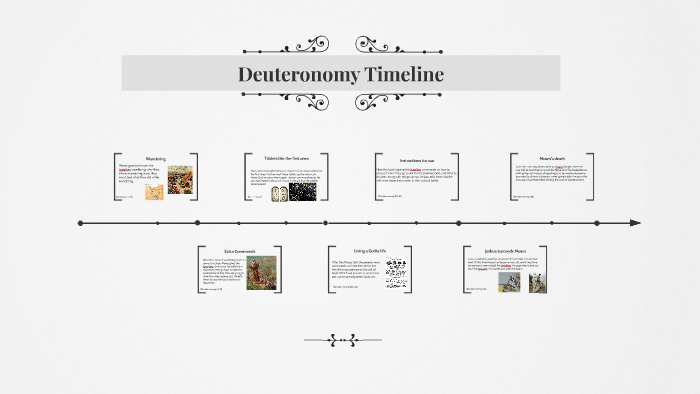
\includegraphics[scale=.7, angle=0]{05OT-Deuteronomy/References/AndrewSmithDeuteronomyTimeline.png}
%\caption[Deuteronomy Timeline by Andrew Smith]{Deuteronomy Timeline by Andrew %Smith}
%\label{fig:Deuteronomy Timeline by Andrew Smith}
%\end{center}
%\end{figure}

\newpage
\begin{figure}
\begin{center}
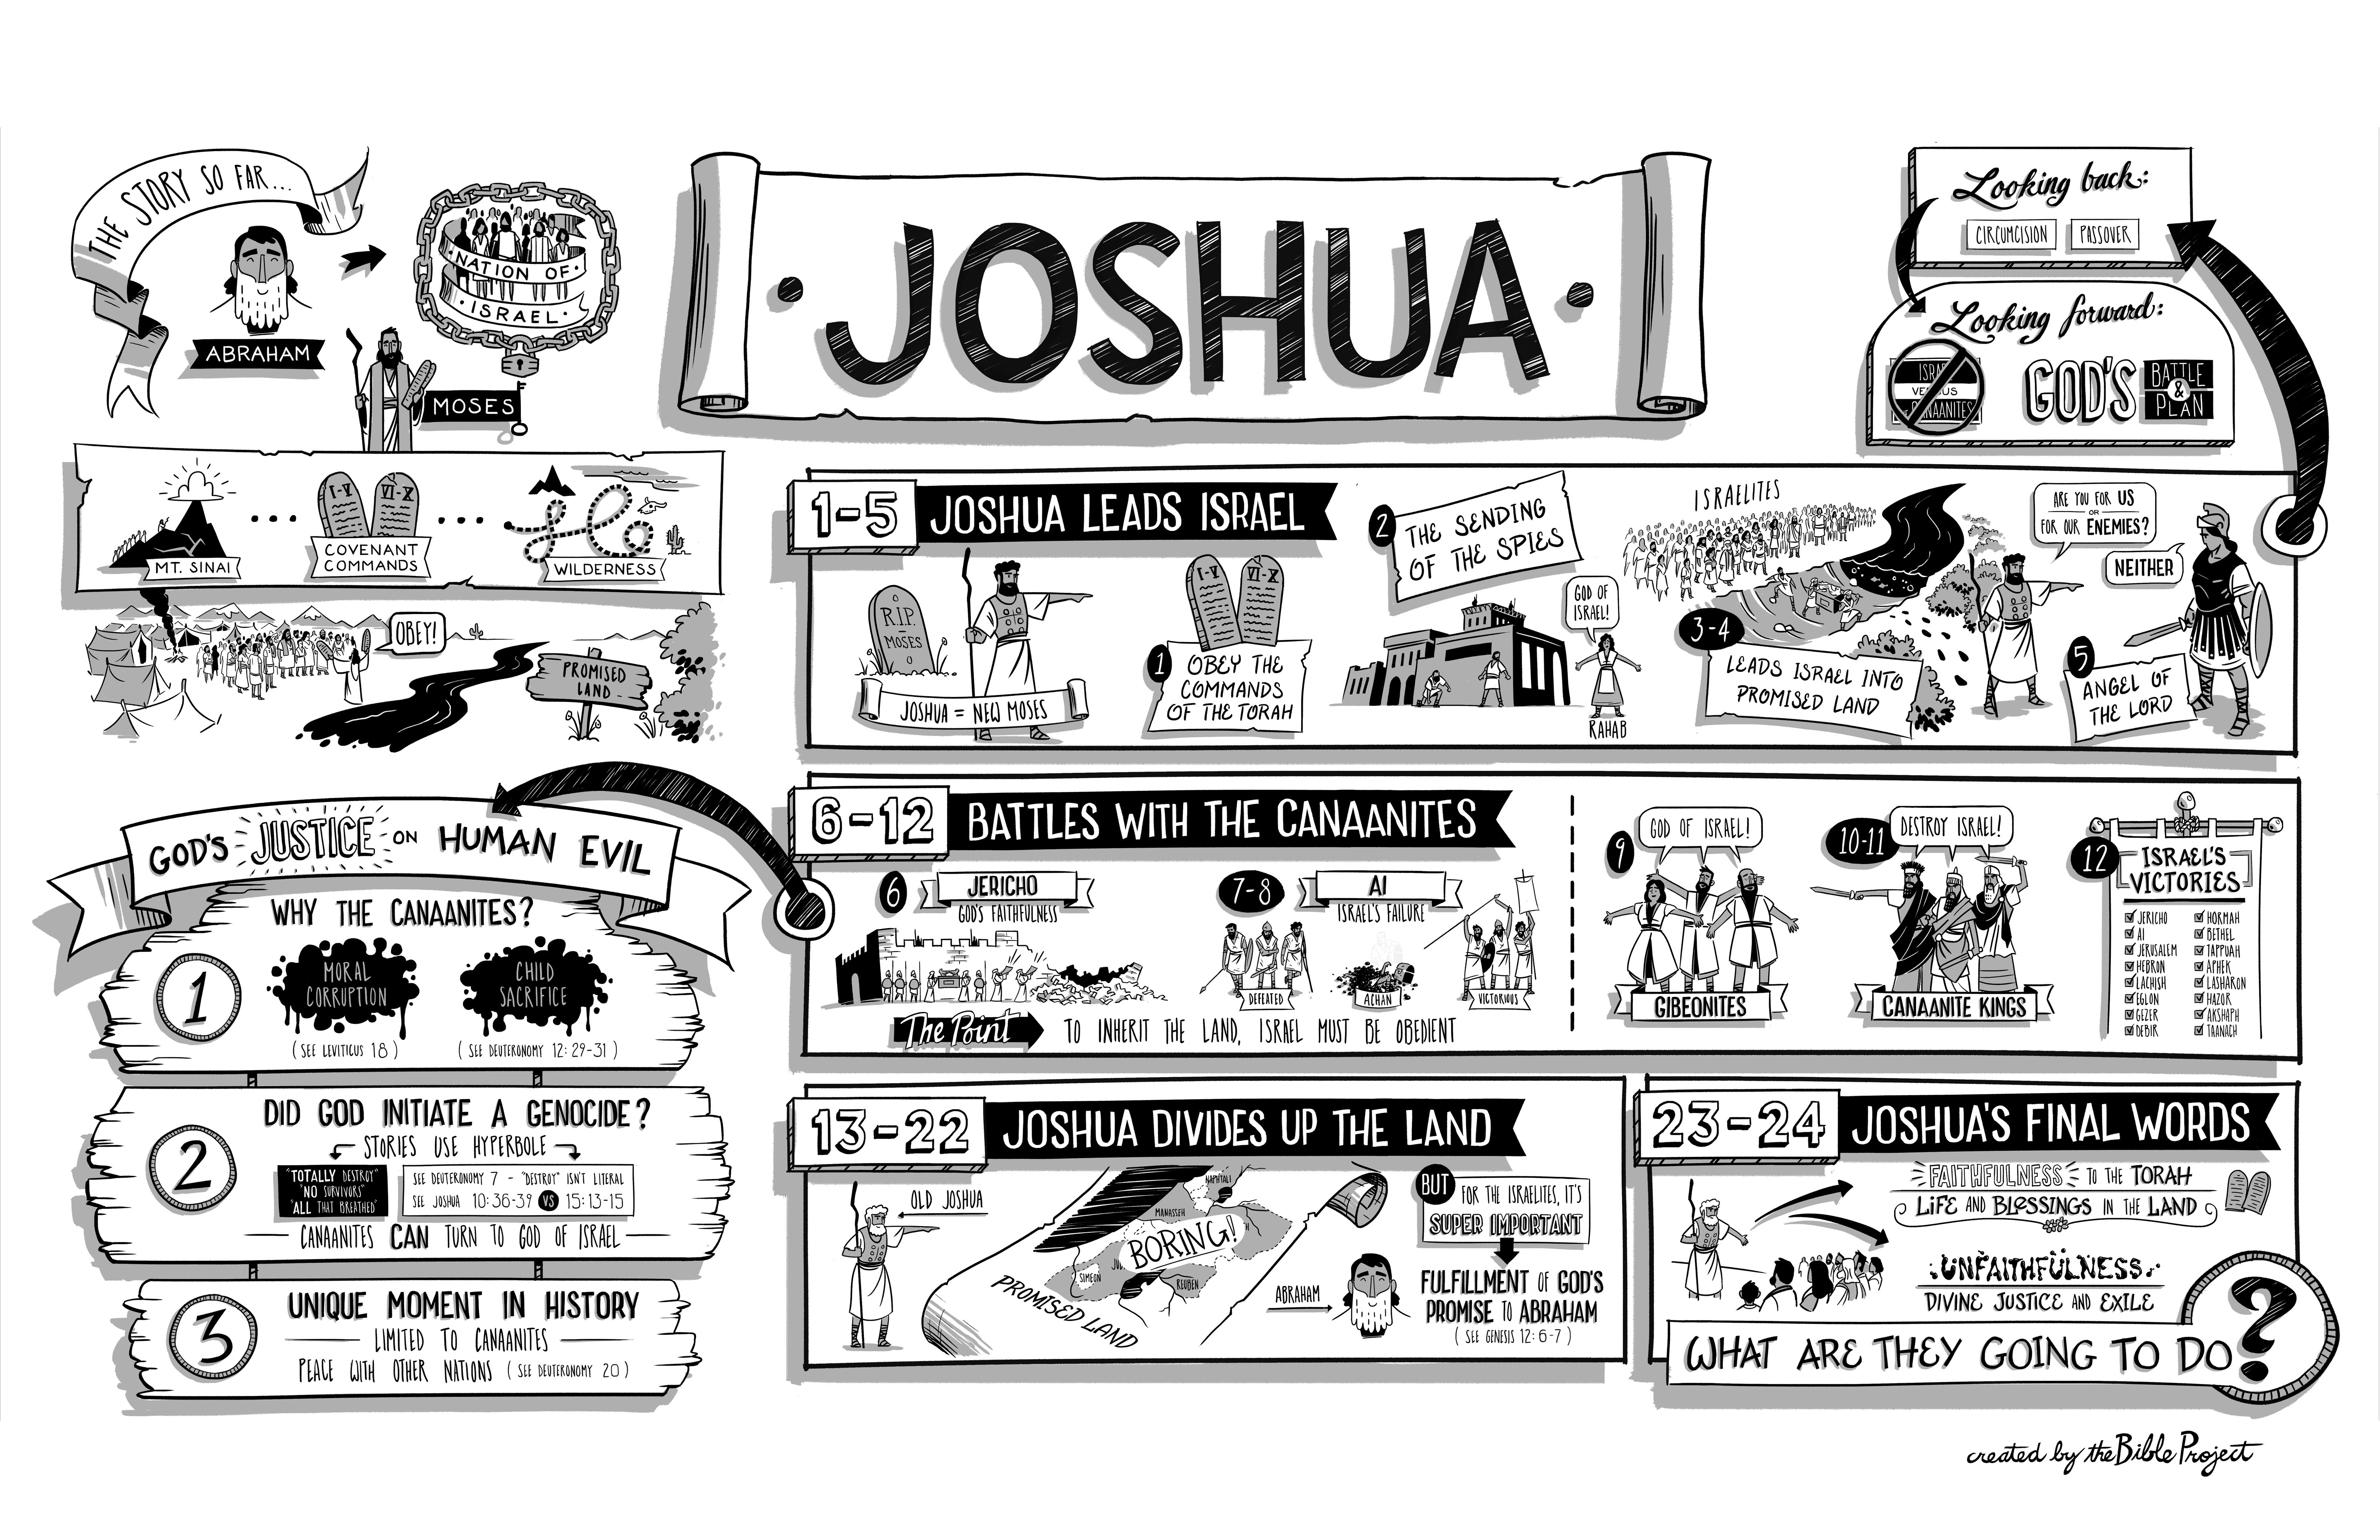
\includegraphics[scale=0.5, angle=90]{06OT-Joshua/References/1.BibleProject-Joshua.jpg}
\caption[Joshua from the Bible Project]{Joshua from the Bible Project}
\label{fig:Joshua from the Bible Project}
\end{center}
\end{figure}

\newpage
\begin{figure}
\begin{center}
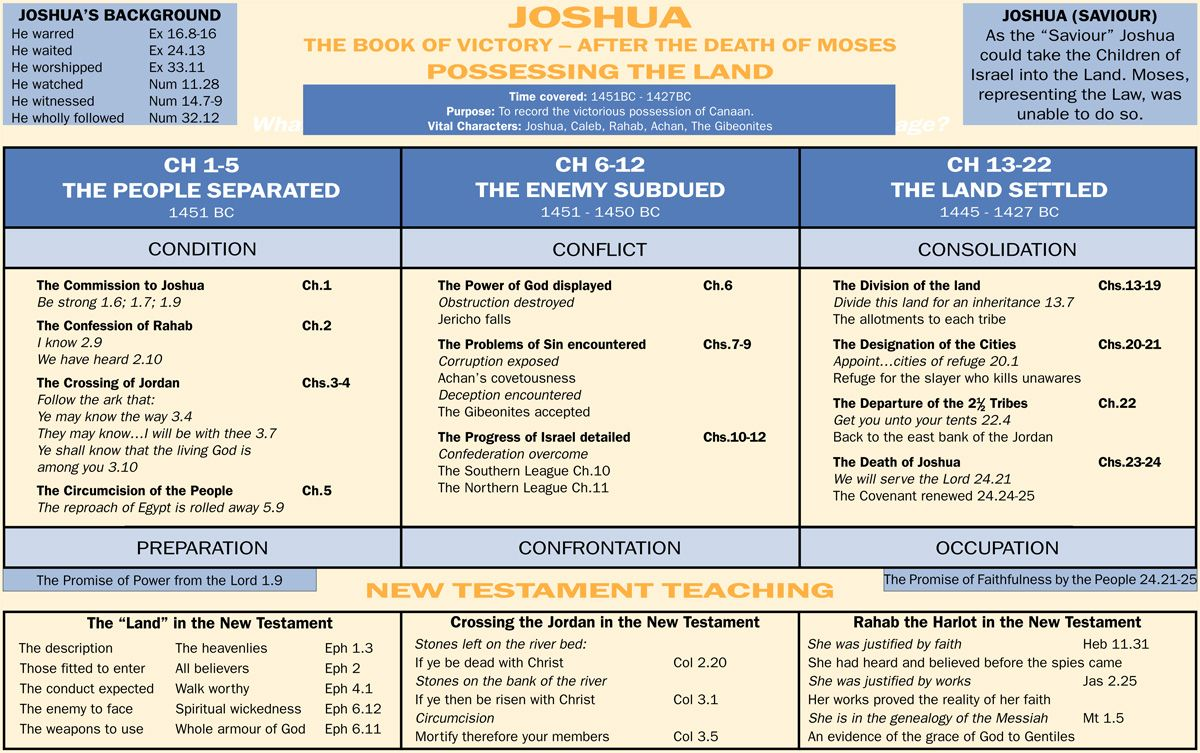
\includegraphics[scale=0.5, angle=90]{06OT-Joshua/References/2.JohnGrant-Joshua.jpg}
\caption[Joshua from John Grant]{Joshua from John Grant}
\label{fig:Joshua from John Grant}
\end{center}
\end{figure}

\newpage
\begin{figure}
\begin{center}
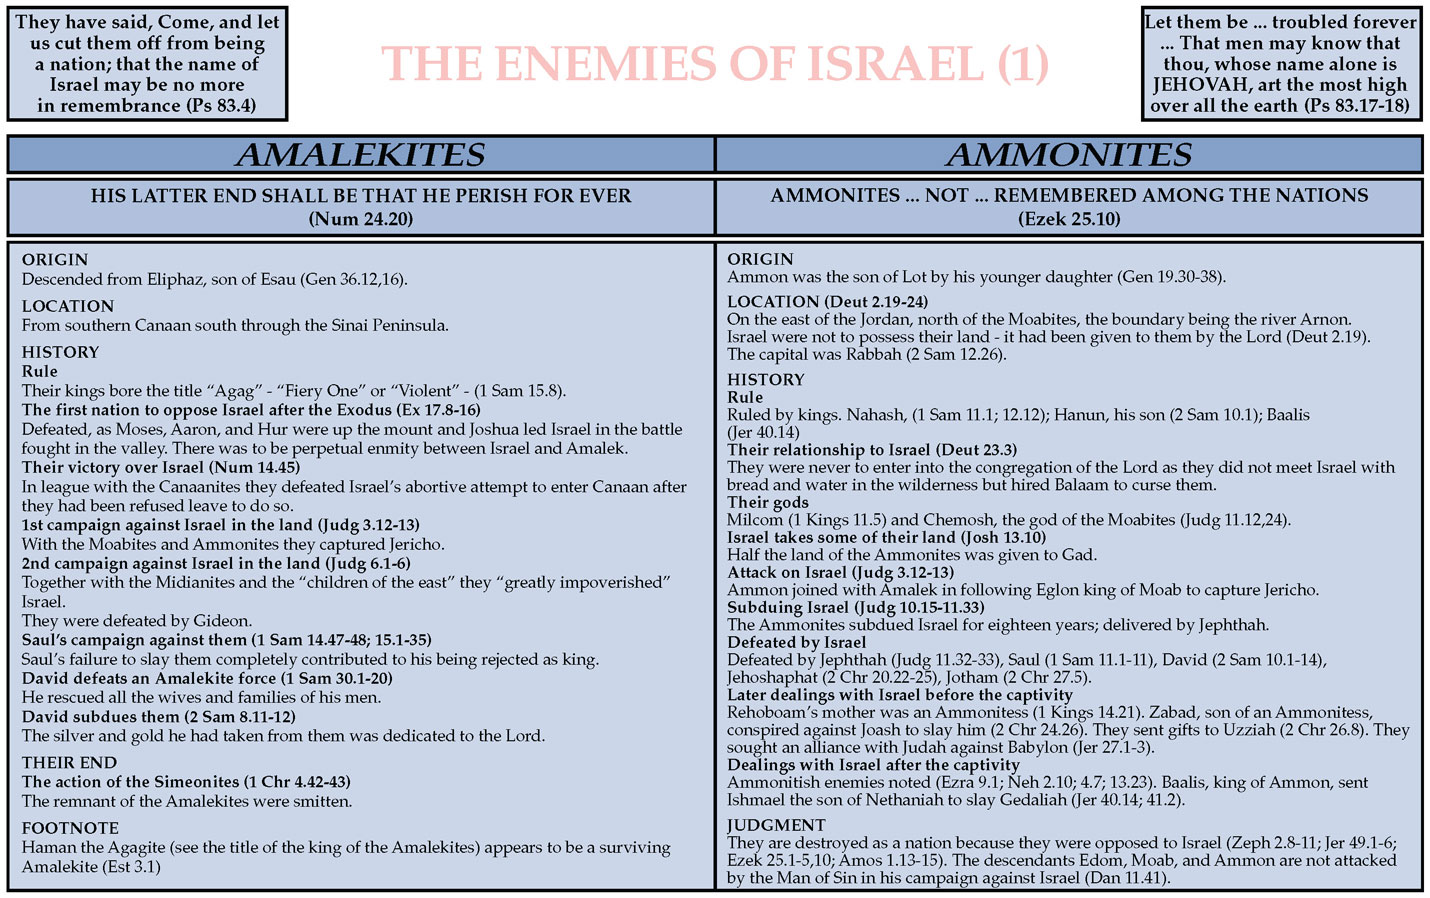
\includegraphics[scale=0.4, angle=90]{06OT-Joshua/References/3.EnemiesOfIsrael1.jpg}
\caption[Enemies of Israel 1]{Enemies of Israel 1}
\label{fig:Enemies of Israel 1}
\end{center}
\end{figure}

\newpage
\begin{figure}
\begin{center}
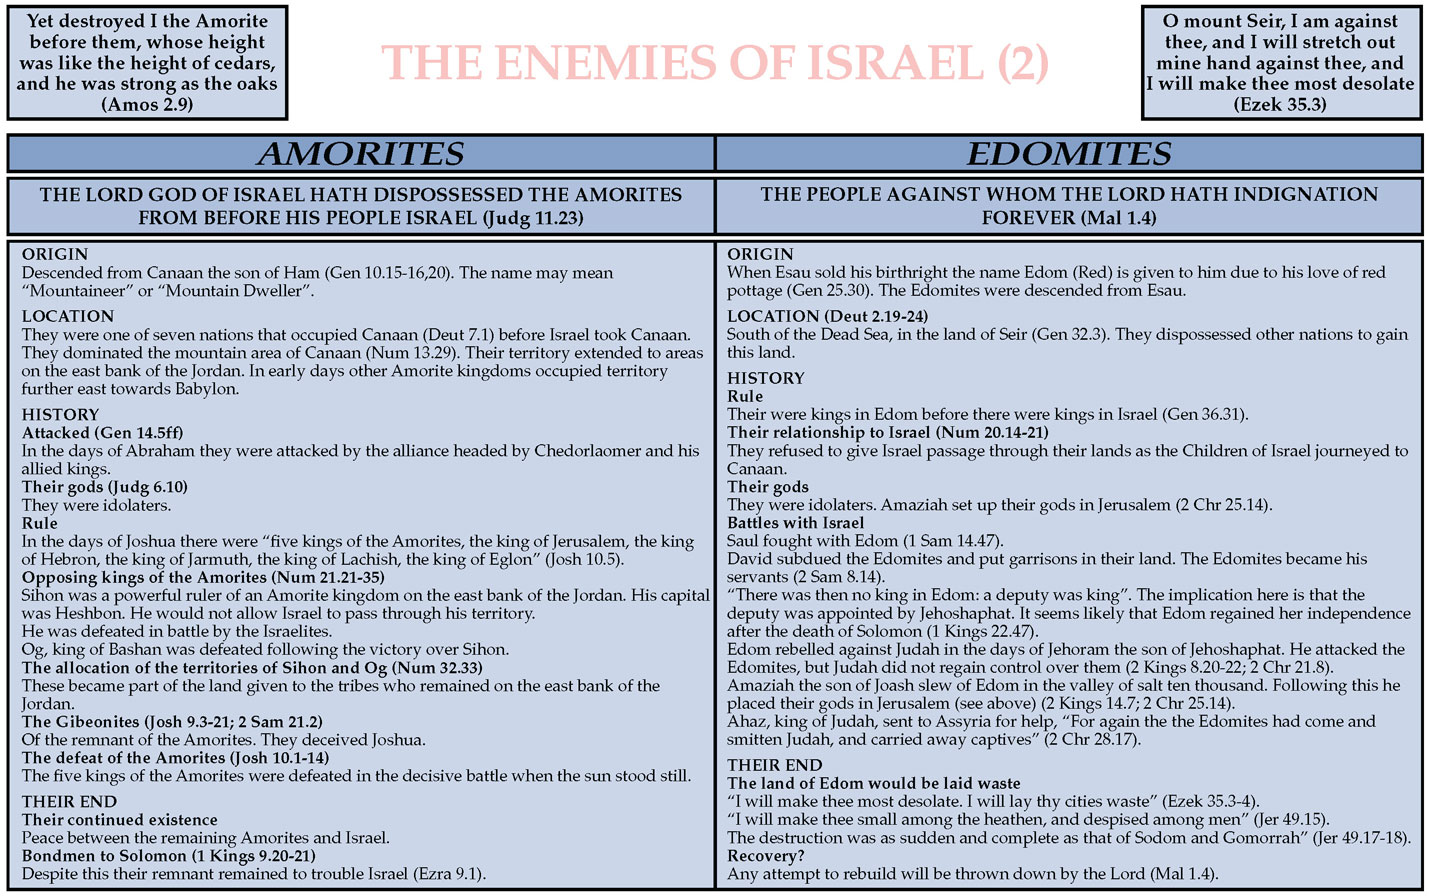
\includegraphics[scale=0.4, angle=90]{06OT-Joshua/References/4.EnemiesOfIsrael2.jpg}
\caption[Enemies of Israel 2]{Enemies of Israel 2}
\label{fig:Enemies of Israel 2}
\end{center}
\end{figure}

\newpage
\begin{figure}
\begin{center}
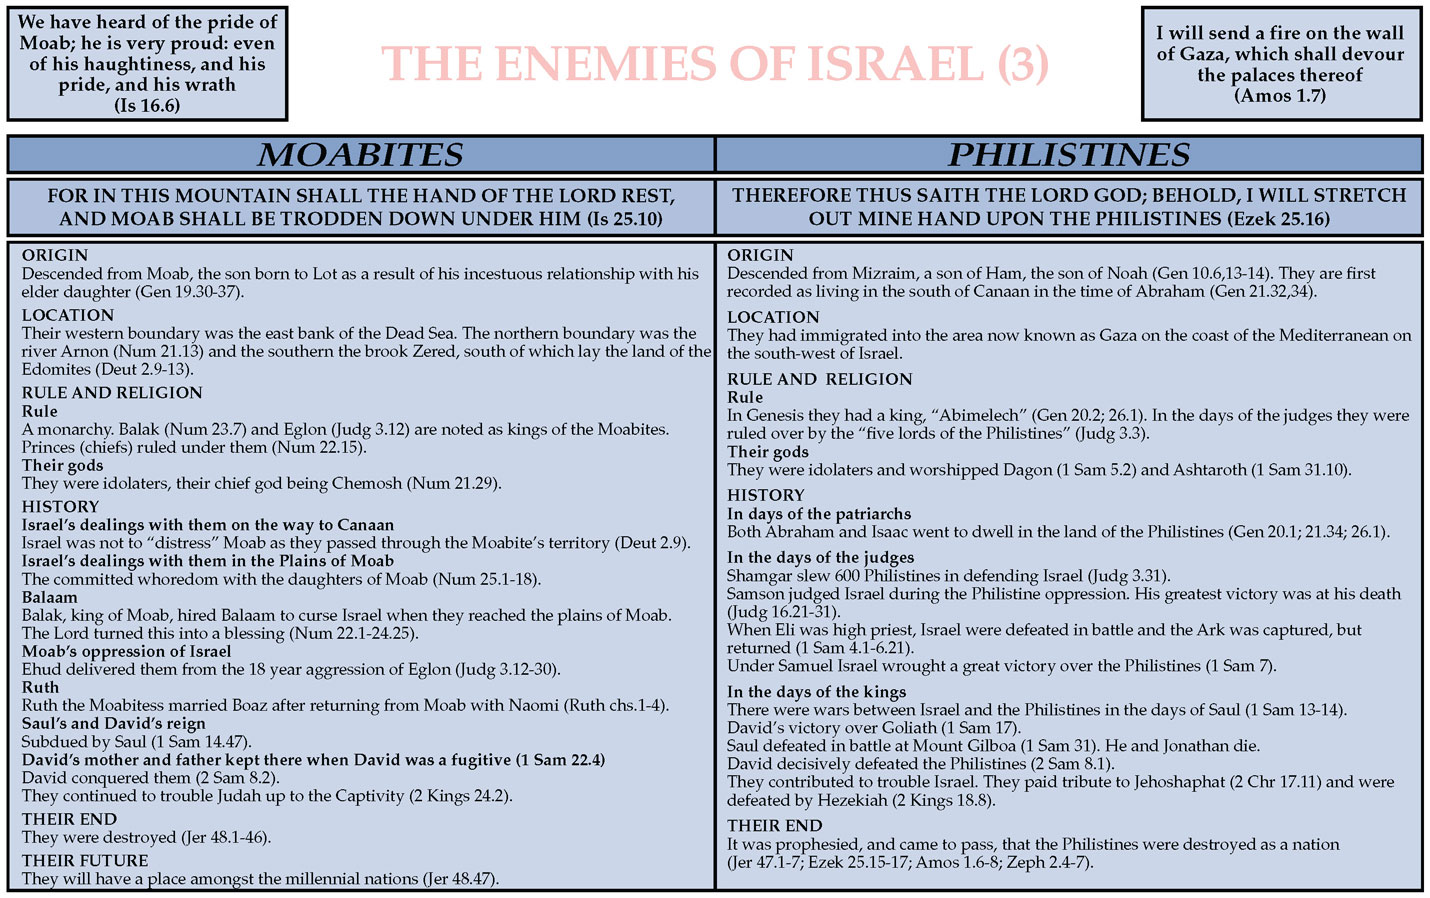
\includegraphics[scale=0.4, angle=90]{06OT-Joshua/References/5.EnemiesOfIsrael3.jpg}
\caption[Enemies of Israel 3]{Enemies of Israel 3}
\label{fig:Enemies of Israel 3}
\end{center}
\end{figure}

\newpage
\begin{figure}
\begin{center}
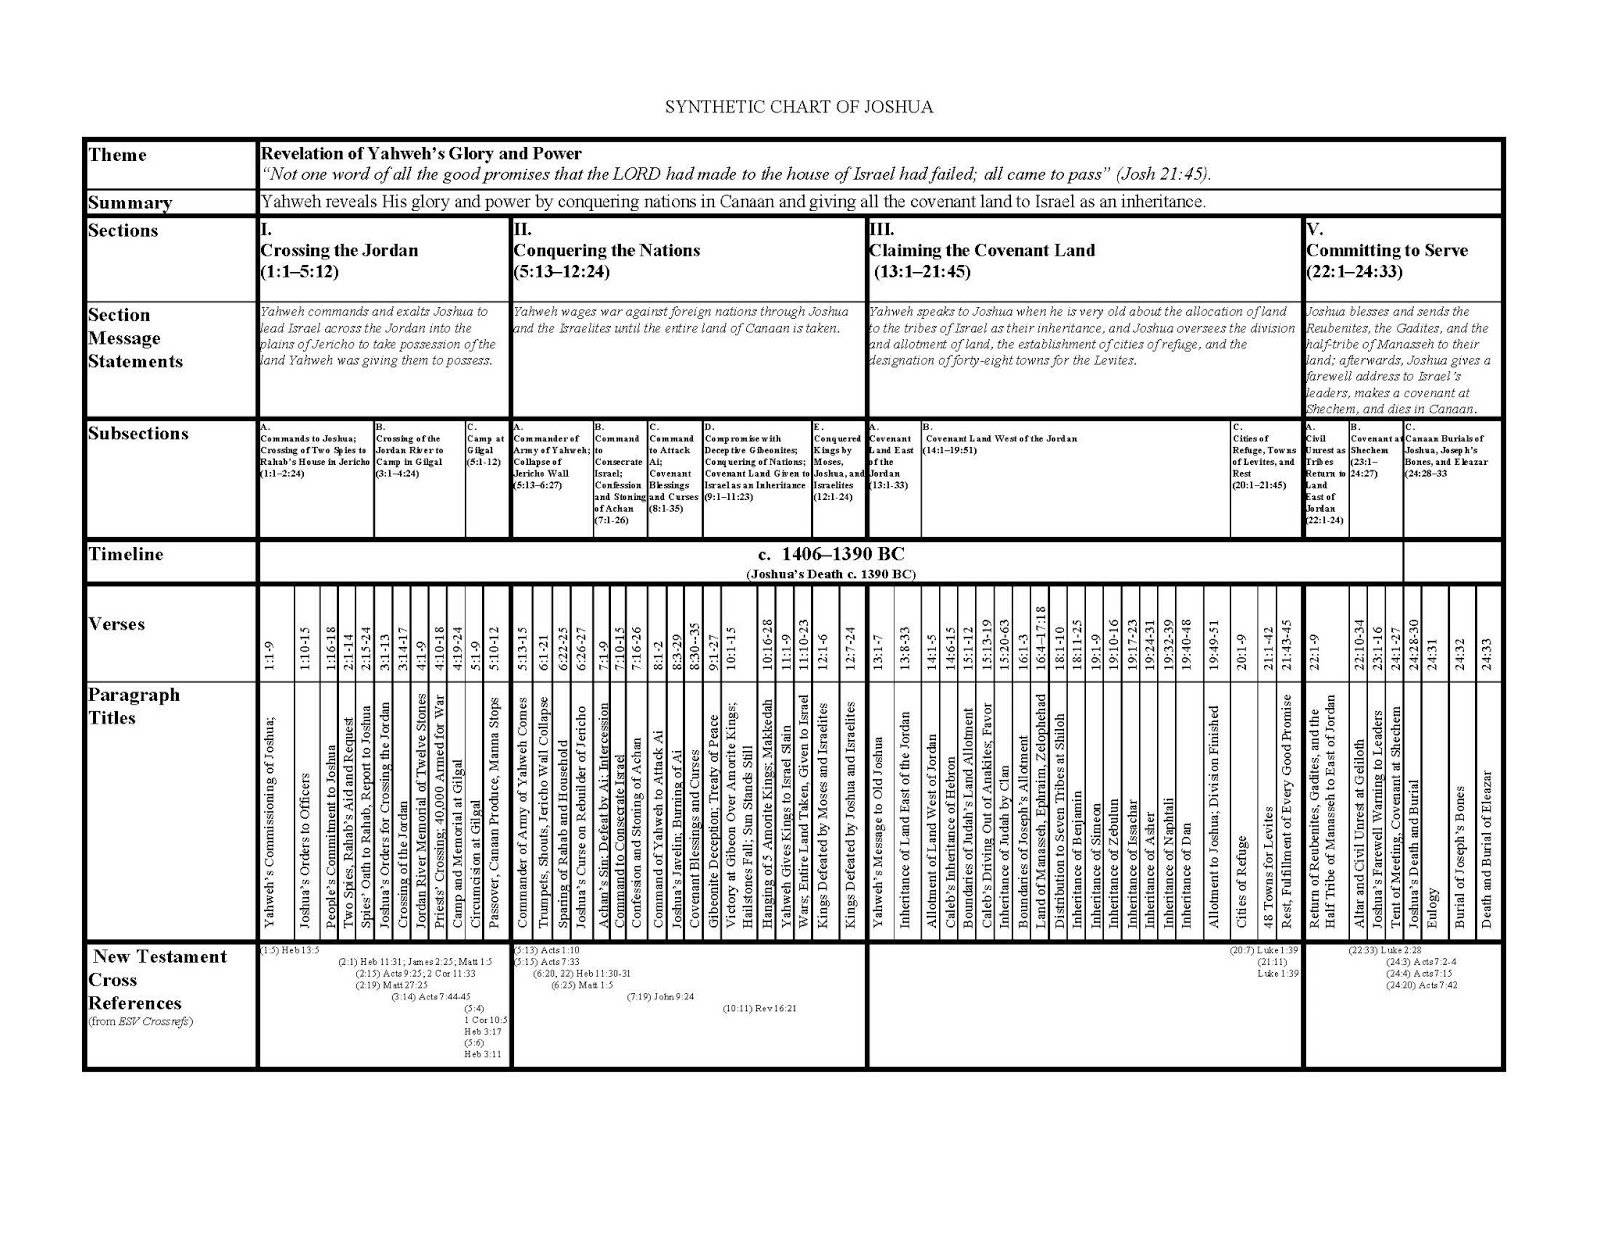
\includegraphics[scale=.4, angle=90]{06OT-Joshua/References/6.SyntheticChartofJoshua.jpg}
\caption[Synthetic Chart of Joshua]{Synthetic Chart of Joshua}
\label{fig:Synthetic Chart of Joshua}
\end{center}
\end{figure}


\newpage
\begin{figure}
\begin{center}
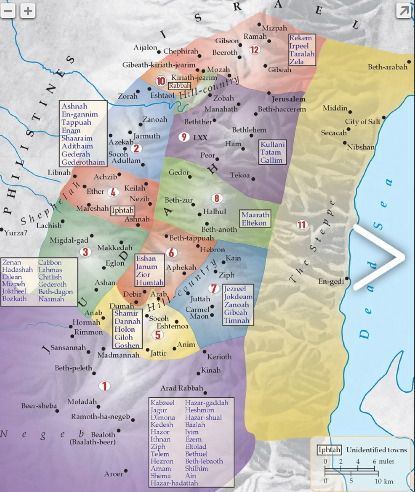
\includegraphics[scale=1, angle=0]{06OT-Joshua/References/7.WestSideOfDeadSea.jpg}
\caption[The West Side of the Dead Sea]{The West Side of the Dead Sea}
\label{fig:The West Side of the Dead Sea}
\end{center}
\end{figure}


\newpage
\begin{figure}
\begin{center}
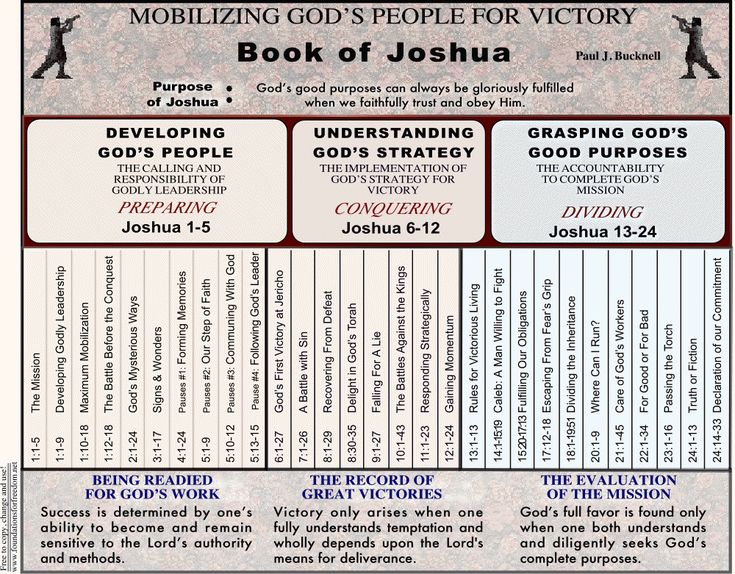
\includegraphics[scale=0.75, angle=90]{06OT-Joshua/References/8.Bucknell-Joshua.jpg}
\caption[Joshua from Bucknell]{Joshua from Bucknell}
\label{fig:Joshua from Bucknell}
\end{center}
\end{figure}


\newpage
\begin{figure}
\begin{center}
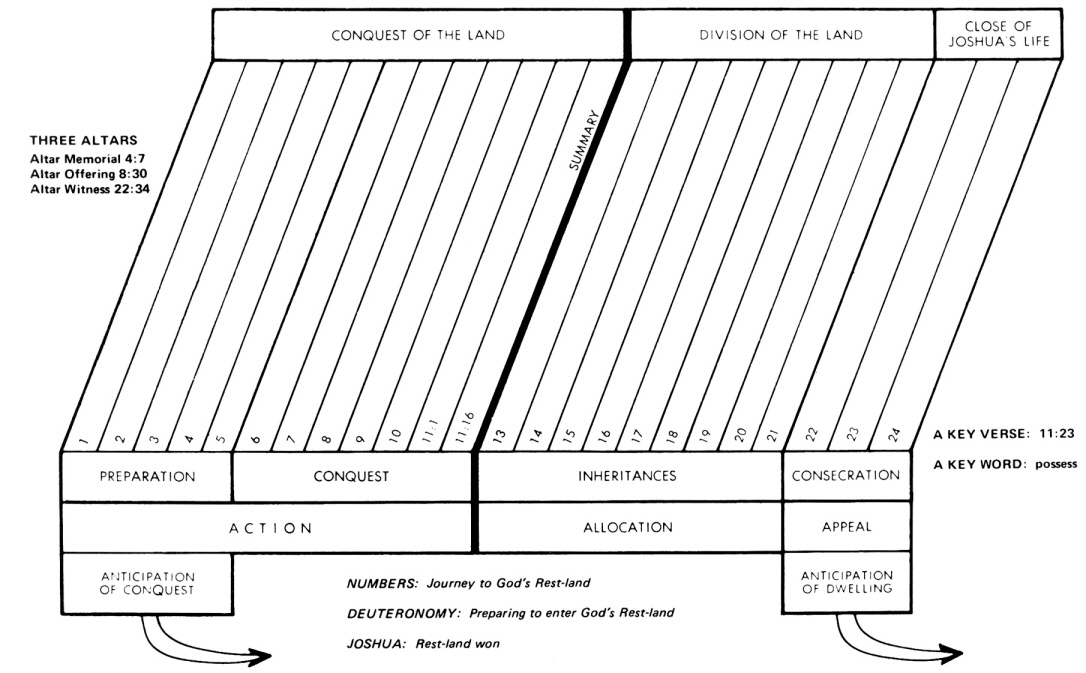
\includegraphics[scale=2, angle=90]{06OT-Joshua/References/9.Jensen-Joshua.png}
\caption[Joshua from Jensen]{Joshua from Jensen}
\label{fig:Joshua from Jensen}
\end{center}
\end{figure}


\newpage
\begin{figure}
\begin{center}
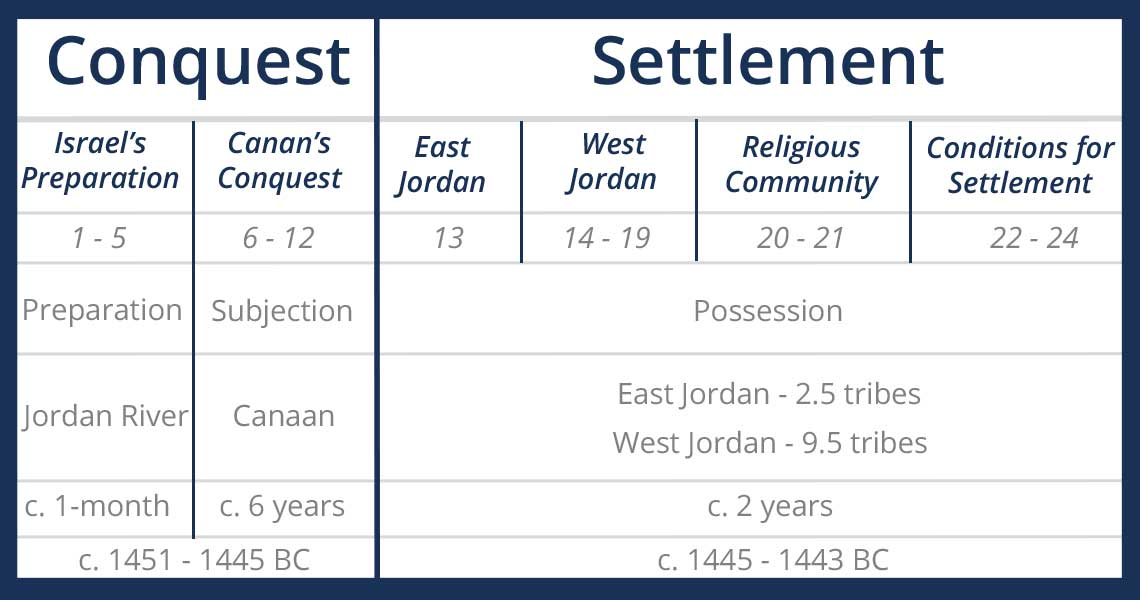
\includegraphics[scale=.5, angle=90]{06OT-Joshua/References/10.Bible-Brief-Joshua.jpg}
\caption[Bible Brief for Joshua]{Bible Brief for Joshua}
\label{fig:Bible Brief for Joshua}
\end{center}
\end{figure}

\newpage
\begin{figure}
\begin{center}
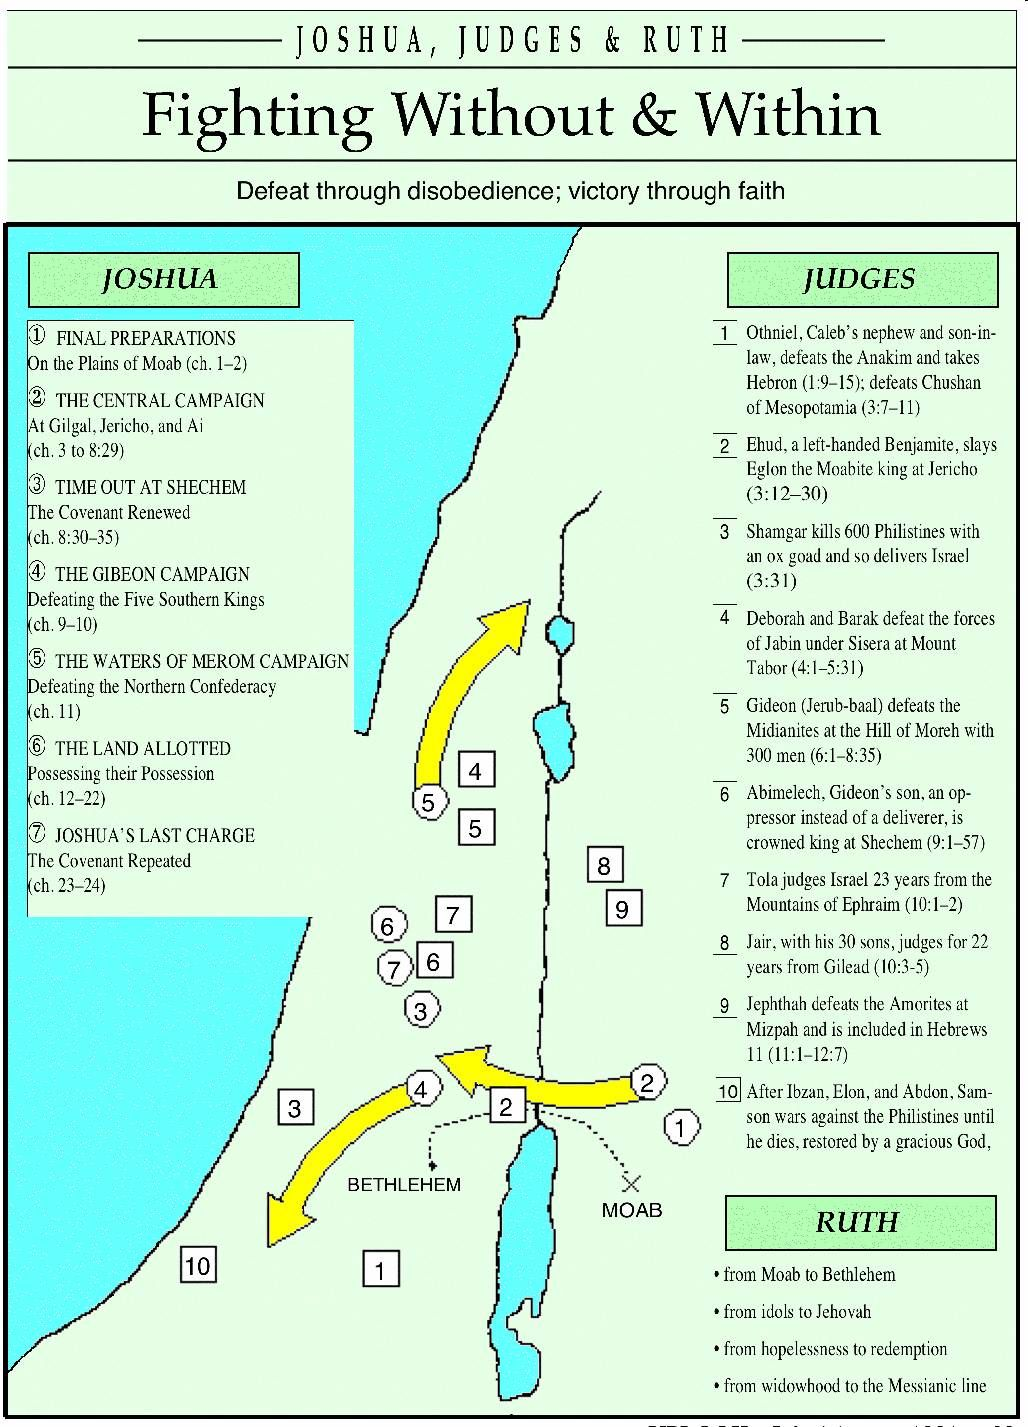
\includegraphics[scale=.5, angle=0]{06OT-Joshua/References/11.FightingInJoshuaAndJudges.jpg}
\caption[The Fighting in Joshua and Judges]{The Fighting in Joshua and Judges}
\label{fig:The Fighting in Joshua and Judges}
\end{center}
\end{figure}

\newpage
\begin{figure}
\begin{center}
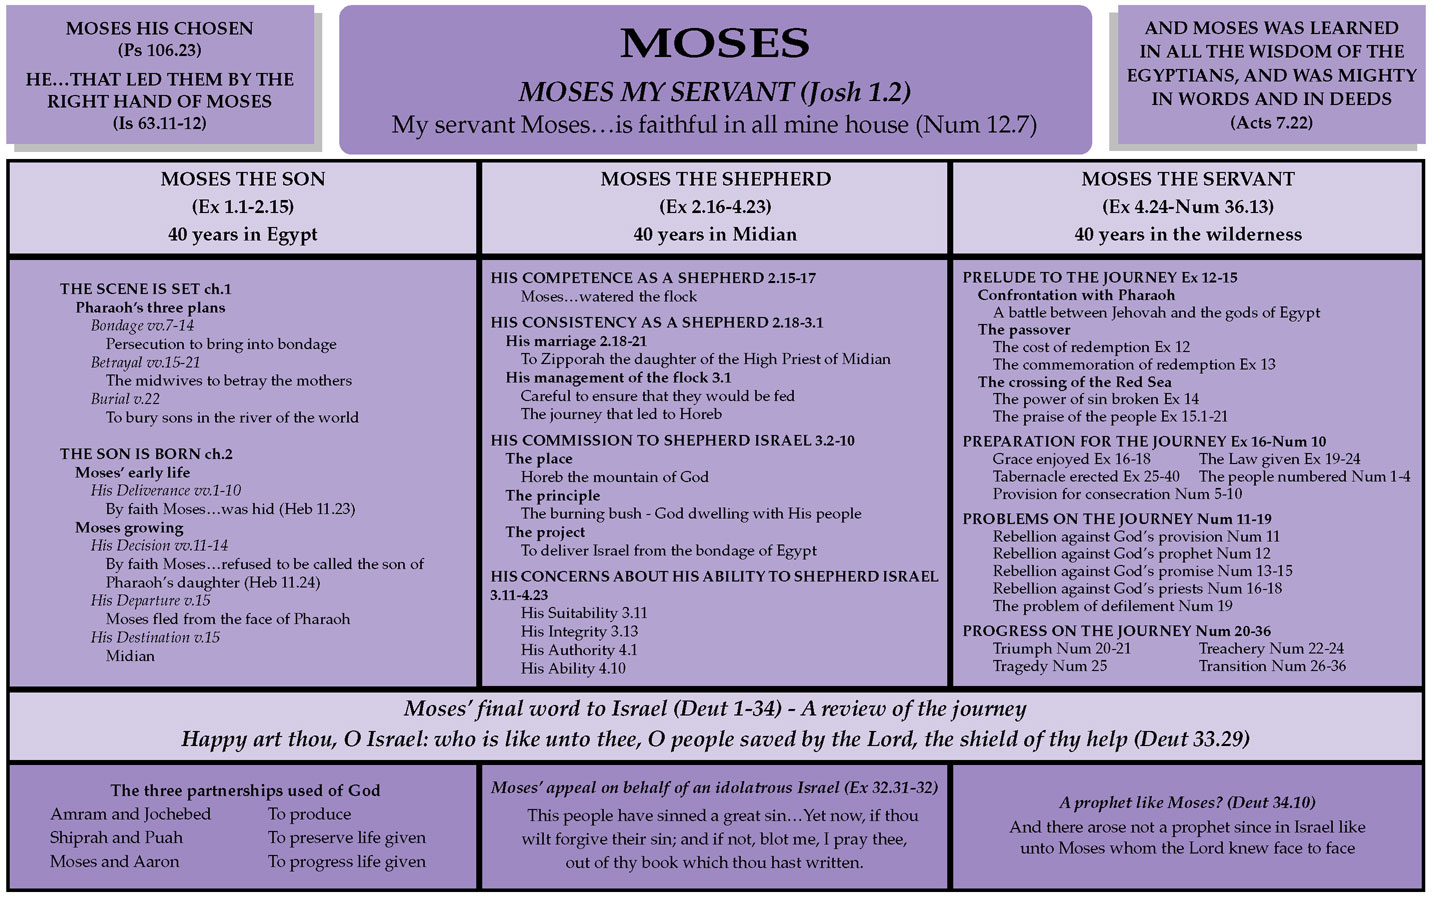
\includegraphics[scale=.4, angle=90]{06OT-Joshua/References/12.JohnGrantMoses.jpg}
\caption[Moses from John Grant]{Moses from John Grant}
\label{fig:Moses from John Grant}
\end{center}
\end{figure}








\chapter{Joshua 7}

\begin{figure}
  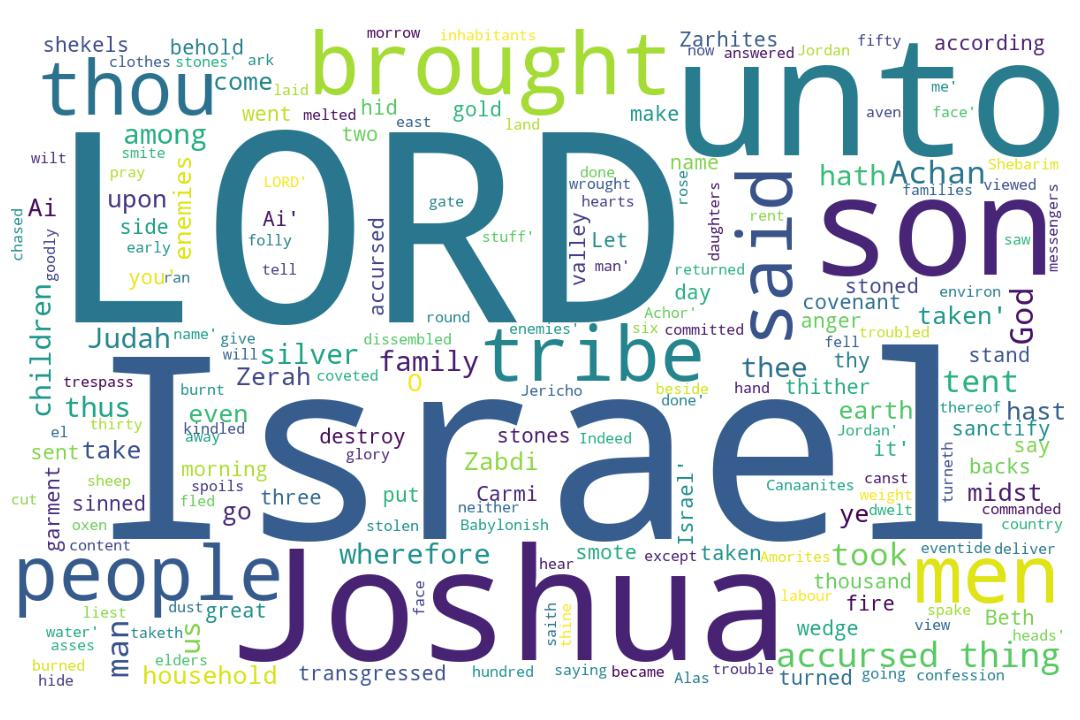
\includegraphics[width=\linewidth]{06OT-Joshua/Joshua7-WordCloud.jpg}
  \caption{Joshua 7 Word Cloud}
  \label{fig:Joshua 7Word Cloud}
\end{figure}

\marginpar{\scriptsize \centering \fcolorbox{bone}{lime}{\textbf{ACHIN FOR A BRUSIN'}}\\ (Joshua 7)

\begin{compactenum}[I.][8]

\item A \textbf{Pernicious Defiling}
\item A \textbf{Painful Defeat} \index[scripture]{Joshua!Jsh 07:04}  (Jsh 7:4) 
\item A \textbf{Public Declaration} \index[scripture]{Joshua!Jsh 07:20}  (Jsh 7:20) 
\item \textbf{Polluted Desire} \index[scripture]{Joshua!Jsh 07:21}  (Jsh 7:21) 
\item A \textbf{Personal Decision} \index[scripture]{Joshua!Jsh 07:21}  (Jsh 7:21) 
\item \textbf{Disproportionate Destruction} \index[scripture]{Joshua!Jsh 07:24}  (Jsh 7:24) 
\item A \textbf{Purifying Death} \index[scripture]{Joshua!Jsh 07:25}  (Jsh 7:25) 
\end{compactenum}}




\footnote{\textcolor[rgb]{0.00,0.25,0.00}{\hyperlink{TOC}{Return to end of Table of Contents.}}}\footnote{\href{https://audiobible.com/bible/joshua_7.html}{\textcolor[cmyk]{0.99998,1,0,0}{Joshua 7 Audio}}}\textcolor[cmyk]{0.99998,1,0,0}{But the children of Israel committed a trespass in the accursed thing: for Achan, the son of Carmi, the son of Zabdi, the son of Zerah, of the tribe of Judah, took of the accursed thing: and the anger of \fcolorbox{bone}{bone}{the LORD} was kindled against the children of Israel.}
[2] \textcolor[cmyk]{0.99998,1,0,0}{And Joshua sent men from Jericho to Ai, which \emph{is} beside Beth-aven, on the east side of Beth-el, and spake \fcolorbox{bone}{bone}{unto} \fcolorbox{bone}{bone}{them}, saying, Go up and view the country. And the men went up and viewed Ai.}
[3] \textcolor[cmyk]{0.99998,1,0,0}{And they returned to Joshua, and said \fcolorbox{bone}{bone}{unto} him, Let not all the people go up; but let about two or three thousand men go up and smite Ai; \emph{and} make not all the people to labour thither; for they \emph{are} \emph{but} few.}
[4] \textcolor[cmyk]{0.99998,1,0,0}{So there went up thither of the people about three thousand men: and they fled before the men of Ai.}
[5] \textcolor[cmyk]{0.99998,1,0,0}{And the men of Ai smote of \fcolorbox{bone}{bone}{them} about thirty and six men: for they chased \fcolorbox{bone}{bone}{them} \emph{from} before the gate \emph{even} \fcolorbox{bone}{bone}{unto} Shebarim, and smote \fcolorbox{bone}{bone}{them} in the going down: wherefore the hearts of the people melted, and became as water.}\\
\\
\P \textcolor[cmyk]{0.99998,1,0,0}{And Joshua rent his clothes, and fell to the earth upon his face before the ark of \fcolorbox{bone}{bone}{the LORD} until the eventide, he and the elders of Israel, and put dust upon their heads.}
[7] \textcolor[cmyk]{0.99998,1,0,0}{And Joshua said, Alas, O Lord GOD, wherefore hast thou at all brought this people over Jordan, to deliver us into the hand of the Amorites, to destroy us? would to God we had been content, and dwelt on the other side Jordan!}
[8] \textcolor[cmyk]{0.99998,1,0,0}{O Lord, what \fcolorbox{bone}{bone}{shall} I say, when Israel turneth their backs before their enemies!}
[9] \textcolor[cmyk]{0.99998,1,0,0}{For the Canaanites and all the inhabitants of the land \fcolorbox{bone}{bone}{shall} hear \emph{of} \emph{it}, and \fcolorbox{bone}{bone}{shall} environ us round, and cut off our name from the earth: and what wilt thou do \fcolorbox{bone}{bone}{unto} thy great name?}\\
\\
\P \textcolor[cmyk]{0.99998,1,0,0}{And \fcolorbox{bone}{bone}{the LORD} said \fcolorbox{bone}{bone}{unto} Joshua, Get thee up; wherefore liest thou thus upon thy face?}
[11] \textcolor[cmyk]{0.99998,1,0,0}{Israel hath sinned, and they have also transgressed my covenant which I commanded \fcolorbox{bone}{bone}{them}: for they have even taken of the accursed thing, and have also stolen, and dissembled also, and they have put \emph{it} even among their own stuff.}
[12] \textcolor[cmyk]{0.99998,1,0,0}{Therefore the children of Israel could not stand before their enemies, \emph{but} turned \emph{their} backs before their enemies, because they were accursed: neither will I be with you any more, except ye destroy the accursed from among you.}
[13] \textcolor[cmyk]{0.99998,1,0,0}{Up, sanctify the people, and say, Sanctify yourselves against to morrow: for thus saith \fcolorbox{bone}{bone}{the LORD} God of Israel, \emph{There} \emph{is} an accursed thing in the midst of thee, O Israel: thou canst not stand before thine enemies, until ye take away the accursed thing from among you.}
[14] \textcolor[cmyk]{0.99998,1,0,0}{In the morning therefore ye \fcolorbox{bone}{bone}{shall} be brought according to your tribes: and it \fcolorbox{bone}{bone}{shall} be, \emph{that} the tribe which \fcolorbox{bone}{bone}{the LORD} taketh \fcolorbox{bone}{bone}{shall} come according to the families \emph{thereof}; and the family which \fcolorbox{bone}{bone}{the LORD} \fcolorbox{bone}{bone}{shall} take \fcolorbox{bone}{bone}{shall} come by households; and the household which \fcolorbox{bone}{bone}{the LORD} \fcolorbox{bone}{bone}{shall} take \fcolorbox{bone}{bone}{shall} come man by man.}
[15] \textcolor[cmyk]{0.99998,1,0,0}{And it \fcolorbox{bone}{bone}{shall} be, \emph{that} he that is taken with the accursed thing \fcolorbox{bone}{bone}{shall} be burnt with fire, he and all that he hath: because he hath transgressed the covenant of \fcolorbox{bone}{bone}{the LORD}, and because he hath wrought folly in Israel.}\\
\\
\P \textcolor[cmyk]{0.99998,1,0,0}{So Joshua rose up early in the morning, and brought Israel by their tribes; and the tribe of Judah was taken:}
[17] \textcolor[cmyk]{0.99998,1,0,0}{And he brought the family of Judah; and he took the family of the Zarhites: and he brought the family of the Zarhites man by man; and Zabdi was taken:}
[18] \textcolor[cmyk]{0.99998,1,0,0}{And he brought his household man by man; and Achan, the son of Carmi, the son of Zabdi, the son of Zerah, of the tribe of Judah, was taken.}
[19] \textcolor[cmyk]{0.99998,1,0,0}{And Joshua said \fcolorbox{bone}{bone}{unto} Achan, My son, give, I pray thee, glory to \fcolorbox{bone}{bone}{the LORD} God of Israel, and make confession \fcolorbox{bone}{bone}{unto} him; and tell me now what thou hast done; hide \emph{it} not from me.}
[20] \textcolor[cmyk]{0.99998,1,0,0}{And Achan answered Joshua, and said, Indeed I have sinned against \fcolorbox{bone}{bone}{the LORD} God of Israel, and thus and thus have I done:}
[21] \textcolor[cmyk]{0.99998,1,0,0}{When I saw among the spoils a goodly Babylonish garment, and two hundred shekels of silver, and a wedge of gold of fifty shekels weight, then I coveted \fcolorbox{bone}{bone}{them}, and took \fcolorbox{bone}{bone}{them}; and, behold, they \emph{are} hid in the earth in the midst of my tent, and the silver under it.}\\
\\
\P \textcolor[cmyk]{0.99998,1,0,0}{So Joshua sent messengers, and they ran \fcolorbox{bone}{bone}{unto} the tent; and, behold, \emph{it} \emph{was} hid in his tent, and the silver under it.}
[23] \textcolor[cmyk]{0.99998,1,0,0}{And they took \fcolorbox{bone}{bone}{them} out of the midst of the tent, and brought \fcolorbox{bone}{bone}{them} \fcolorbox{bone}{bone}{unto} Joshua, and \fcolorbox{bone}{bone}{unto} all the children of Israel, and laid \fcolorbox{bone}{bone}{them} out before \fcolorbox{bone}{bone}{the LORD}.}
[24] \textcolor[cmyk]{0.99998,1,0,0}{And Joshua, and all Israel with him, took Achan the son of Zerah, and the silver, and the garment, and the wedge of gold, and his sons, and his daughters, and his oxen, and his asses, and his sheep, and his tent, and all that he had: and they brought \fcolorbox{bone}{bone}{them} \fcolorbox{bone}{bone}{unto} the valley of Achor.}
[25] \textcolor[cmyk]{0.99998,1,0,0}{And Joshua said, Why hast thou troubled us? \fcolorbox{bone}{bone}{the LORD} \fcolorbox{bone}{bone}{shall} trouble thee this day. And all Israel stoned him with stones, and burned \fcolorbox{bone}{bone}{them} with fire, after they had stoned \fcolorbox{bone}{bone}{them} with stones.}
[26] \textcolor[cmyk]{0.99998,1,0,0}{And they raised over him a great heap of stones \fcolorbox{bone}{bone}{unto} this day. So \fcolorbox{bone}{bone}{the LORD} turned from the fierceness of his anger. Wherefore the name of that place was called, The valley of Achor, \fcolorbox{bone}{bone}{unto} this day.}
]       



\chapter{Joshua 8}

\begin{figure}
  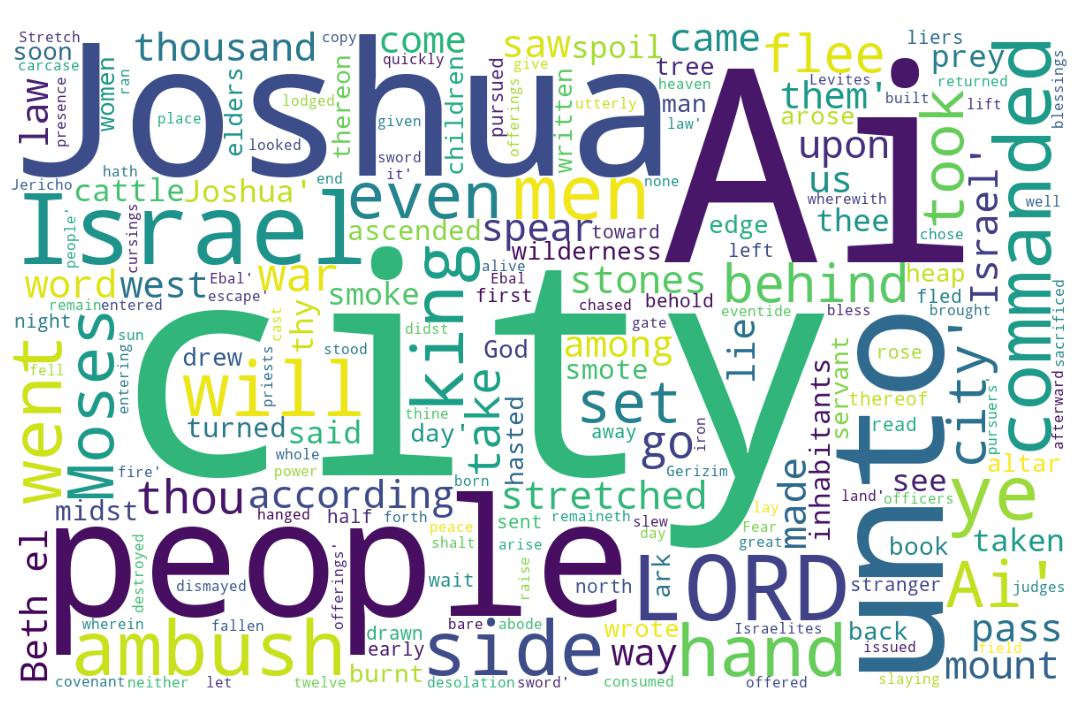
\includegraphics[width=\linewidth]{06OT-Joshua/Joshua8-WordCloud.jpg}
  \caption{Joshua 8 Word Cloud}
  \label{fig:Joshua 8 Word Cloud}
\end{figure}

\marginpar{\scriptsize \centering \fcolorbox{bone}{lime}{\textbf{ACHIN FOR A BRUSIN'}}\\ (Joshua 8)

\begin{compactenum}[I.][8]

	\item A \textbf{Never-Ending Promise} \index[scripture]{Joshua!Jsh 08:01}  (Jsh 8:1) 
	\item \textbf{No Procrastination} \index[scripture]{Joshua!Jsh 08:03}  (Jsh 8:3) 
	\item A \textbf{Nifty Plan} \index[scripture]{Joshua!Jsh 08:07}  (Jsh 8:7) 
	\item An \textbf{Unwise Pursuit} \index[scripture]{Joshua!Jsh 08:16--17}  (Jsh 8:16--17) 
	\item The \textbf{Number who Perished} \index[scripture]{Joshua!Jsh 08:25}  (Jsh 8:25) 
	\item A \textbf{National Presence} \index[scripture]{Joshua!Jsh 08:32}  (Jsh 8:32) 
	\item A \textbf{Notable Publication} \index[scripture]{Joshua!Jsh 08:34}  (Jsh 8:34) 
\end{compactenum}}


\footnote{\textcolor[cmyk]{0.99998,1,0,0}{\hyperlink{TOC}{Return to end of Table of Contents.}}}\textcolor[cmyk]{0.99998,1,0,0}{And the LORD said unto Joshua, Fear not, neither be thou dismayed: take all the \fcolorbox{bone}{bone}{people} of war with thee, and arise, go up to Ai: see, \fcolorbox{bone}{lime}{I have} \fcolorbox{bone}{lime}{given} into thy hand the king of Ai, and his \fcolorbox{bone}{bone}{people}, and his city, and his land:}
[2] \textcolor[cmyk]{0.99998,1,0,0}{And thou shalt do to Ai and her king as thou didst unto Jericho and her king: only the spoil thereof, and the cattle thereof, shall ye take for a prey unto yourselves: lay thee an ambush for the city behind it.}\\
\\
\P \textcolor[cmyk]{0.99998,1,0,0}{So Joshua arose, and all the \fcolorbox{bone}{bone}{people} of war, to go up against Ai: and Joshua chose out thirty thousand mighty men of valour, and \fcolorbox{bone}{lime}{sent them} \fcolorbox{bone}{lime}{away} by night.}
[4] \textcolor[cmyk]{0.99998,1,0,0}{And he commanded them, saying, Behold, ye shall lie in wa\fcolorbox{bone}{bone}{it} against the city, \emph{even} behind the city: go not very far from the city, but be ye all ready:}
[5] \textcolor[cmyk]{0.99998,1,0,0}{And I, and all the \fcolorbox{bone}{bone}{people} that \emph{are} with me, will approach unto the city: and \fcolorbox{bone}{bone}{it} shall come to pass, when they come out against us, as at the first, that we will flee before them,}
[6] \textcolor[cmyk]{0.99998,1,0,0}{(For they will come out after us) till we have drawn them from the city; for they will say, They flee before us, as at the first: therefore we will flee before them.}
[7] \textcolor[cmyk]{0.99998,1,0,0}{Then ye shall rise up from the ambush, and seize upon the city: for the LORD your \fcolorbox{bone}{lime}{God will deliver} \fcolorbox{bone}{bone}{it} into your hand.}
[8] \textcolor[cmyk]{0.99998,1,0,0}{And \fcolorbox{bone}{bone}{it} shall be, when ye have taken the city, \emph{that} ye shall set the city \fcolorbox{bone}{bone}{on} fire: according to the commandment of the LORD shall ye do. See, I have commanded you.}\\
\\
\P \textcolor[cmyk]{0.99998,1,0,0}{Joshua therefore sent them forth: and they went to lie in ambush, and abode between Beth-el and Ai, \fcolorbox{bone}{bone}{on} the west side of Ai: but Joshua lodged that night among the \fcolorbox{bone}{bone}{people}.}
[10] \textcolor[cmyk]{0.99998,1,0,0}{And Joshua rose up early in the morning, and numbered the \fcolorbox{bone}{bone}{people}, and went up, he and the elders of Israel, before the \fcolorbox{bone}{bone}{people} to Ai.}
[11] \textcolor[cmyk]{0.99998,1,0,0}{And all the \fcolorbox{bone}{bone}{people}, \emph{even} \emph{the} \emph{people} of war that \emph{were} with him, went up, and drew nigh, and came before the city, and pitched \fcolorbox{bone}{bone}{on} the north side of Ai: now \emph{there} \emph{was} a valley between them and Ai.}
[12] \textcolor[cmyk]{0.99998,1,0,0}{And he took about five thousand men, and set them to lie in ambush between Beth-el and Ai, \fcolorbox{bone}{bone}{on} the west side of the city.}
[13] \textcolor[cmyk]{0.99998,1,0,0}{And when they had set the \fcolorbox{bone}{bone}{people}, \emph{even} all the host that \emph{was} \fcolorbox{bone}{bone}{on} the north of the city, and their liers in wa\fcolorbox{bone}{bone}{it} \fcolorbox{bone}{bone}{on} the west of the city, Joshua went that night into the midst of the valley.}\\
\\
\P \textcolor[cmyk]{0.99998,1,0,0}{And \fcolorbox{bone}{bone}{it} came to pass, when the king of Ai saw \emph{it}, that they hasted and rose up early, and the men of the city went out against Israel to battle, he and all his \fcolorbox{bone}{bone}{people}, at a time appointed, before the plain; but he wist not that \emph{there} \emph{were} liers in ambush against him behind the city.}
[15] \textcolor[cmyk]{0.99998,1,0,0}{And Joshua and all Israel made as if they were beaten before them, and fled by the way of the wilderness.}
[16] \textcolor[cmyk]{0.99998,1,0,0}{And all the \fcolorbox{bone}{bone}{people} that \emph{were} in Ai were called together to \fcolorbox{bone}{lime}{pursue} after them: and they pursued after Joshua, and were drawn away from the city.}
[17] \textcolor[cmyk]{0.99998,1,0,0}{And there was not a man left in Ai or Beth-el, that went not out after Israel: and they left the city open, and pursued after Israel.}
[18] \textcolor[cmyk]{0.99998,1,0,0}{And the LORD said unto Joshua, Stretch out the spear that \emph{is} in thy hand toward Ai; for I will give \fcolorbox{bone}{bone}{it} into thine hand. And Joshua stretched out the spear that \emph{he} \emph{had} in his hand toward the city.}
[19] \textcolor[cmyk]{0.99998,1,0,0}{And the ambush arose quickly out of their place, and they ran as soon as he had stretched out his hand: and they entered into the city, and took it, and hasted and set the city \fcolorbox{bone}{bone}{on} fire.}
[20] \textcolor[cmyk]{0.99998,1,0,0}{And when the men of Ai looked behind them, they saw, and, behold, the smoke of the city ascended up to heaven, and they had no power to flee this way or that way: and the \fcolorbox{bone}{bone}{people} that fled to the wilderness turned back upon the pursuers.}
[21] \textcolor[cmyk]{0.99998,1,0,0}{And when Joshua and all Israel saw that the ambush had taken the city, and that the smoke of the city ascended, then they turned again, and slew the men of Ai.}
[22] \textcolor[cmyk]{0.99998,1,0,0}{And the other issued out of the city against them; so they were in the midst of Israel, some \fcolorbox{bone}{bone}{on} this side, and some \fcolorbox{bone}{bone}{on} that side: and they smote them, so that they let none of them remain or escape.}
[23] \textcolor[cmyk]{0.99998,1,0,0}{And the king of Ai they took alive, and brought him to Joshua.}
[24] \textcolor[cmyk]{0.99998,1,0,0}{And \fcolorbox{bone}{bone}{it} came to pass, when Israel had made an end of slaying all the inhabitants of Ai in the field, in the wilderness wherein they chased them, and when they were all fallen \fcolorbox{bone}{bone}{on} the edge of the sword, until they were consumed, that all the Israelites returned unto Ai, and smote \fcolorbox{bone}{bone}{it} with the edge of the sword.}
[25] \textcolor[cmyk]{0.99998,1,0,0}{And \emph{so} \fcolorbox{bone}{bone}{it} was, \emph{that} all that fell that day, both of men and women, \emph{were} \fcolorbox{bone}{lime}{twelve thousand}, \emph{even} all the men of Ai.}
[26] \textcolor[cmyk]{0.99998,1,0,0}{For Joshua drew not his hand back, wherewith he stretched out the spear, until he had utterly destroyed all the inhabitants of Ai.}
[27] \textcolor[cmyk]{0.99998,1,0,0}{Only the cattle and the spoil of that city Israel took for a prey unto themselves, according unto the word of the LORD which he commanded Joshua.}
[28] \textcolor[cmyk]{0.99998,1,0,0}{And Joshua burnt Ai, and made \fcolorbox{bone}{bone}{it} an heap for ever, \emph{even} a desolation unto this day.}
[29] \textcolor[cmyk]{0.99998,1,0,0}{And the king of Ai he hanged \fcolorbox{bone}{bone}{on} a tree until eventide: and as soon as the sun was down, Joshua commanded that they should take his carcase down from the tree, and cast \fcolorbox{bone}{bone}{it} at the entering of the gate of the city, and raise thereon a great heap of stones, \emph{that} \emph{remaineth} unto this day.}\\
\\
\P  \textcolor[cmyk]{0.99998,1,0,0}{Then Joshua built an altar unto the LORD God of Israel in mount Ebal,}
[31] \textcolor[cmyk]{0.99998,1,0,0}{As Moses the servant of the LORD commanded the children of Israel, as \fcolorbox{bone}{bone}{it} is written in the book of the law of Moses, an altar of whole stones, over which no man hath lift up \emph{any} iron: and they offered thereon burnt offerings unto the LORD, and sacrificed peace offerings.}\\
\\
\P \textcolor[cmyk]{0.99998,1,0,0}{And he wrote there upon the stones a copy of the law of Moses, which he wrote in the \fcolorbox{bone}{lime}{presence} of the children of Israel.}
[33] \textcolor[cmyk]{0.99998,1,0,0}{And all Israel, and their elders, and officers, and their judges, stood \fcolorbox{bone}{bone}{on} this side the ark and \fcolorbox{bone}{bone}{on} that side before the priests the Levites, which bare the ark of the covenant of the LORD, as well the stranger, as he that was born among them; half of them over against mount Gerizim, and half of them over against mount Ebal; as Moses the servant of the LORD had commanded before, that they should bless the \fcolorbox{bone}{bone}{people} of Israel.}
[34] \textcolor[cmyk]{0.99998,1,0,0}{And afterward \fcolorbox{bone}{lime}{he read} all the words of the law, the blessings and cursings, according to all that is written in the book of the law.}
[35] \textcolor[cmyk]{0.99998,1,0,0}{There was not a word of all that Moses commanded, which Joshua read not before all the congregation of Israel, with the women, and the little ones, and the strangers that were conversant among them.}


\chapter{Joshua 9}

\begin{figure}
  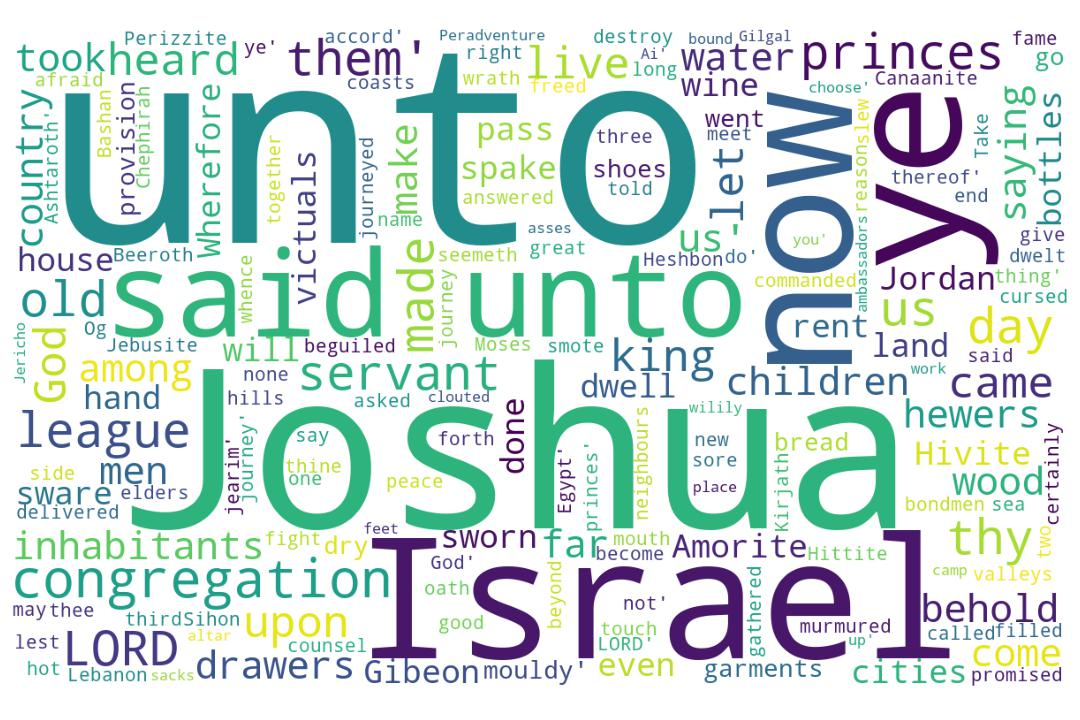
\includegraphics[width=\linewidth]{06OT-Joshua/Joshua9-WordCloud.jpg}
  \caption{Joshua 9 Word Cloud}
  \label{fig:Joshua 9 Word Cloud}
\end{figure}

%%%%%%%%%%%%%%%%%%%%%%%%%%%%%%%%%%%%%%%%%%%%%%%%
\marginpar{\scriptsize \centering \fcolorbox{bone}{lime}{\textbf{A SNEAKY DEAL}}\\ (Joshua 9)
\begin{compactenum}[I.][8]
    \item The \textbf{Dread} \index[scripture]{Joshua!Jsh 09:02} \index[scripture]{Joshua!Jsh 09:24}  (Jsh 9:2, 24) 
    \item The Things that Have been  \textbf{Done} \index[scripture]{Joshua!Jsh 09:03}  
    \item The \textbf{Deception} \index[scripture]{Joshua!Jsh 09:04}  (Jsh 9:4) 
    \item The \textbf{Deal} \index[scripture]{Joshua!Jsh 09:15}  (Jsh 9:15) 
    \item Three \textbf{Days} to Know the Truth \index[scripture]{Joshua!Jsh 09:16--17}  (Jsh 9:16--17) 
    \item \textbf{Drawers and Hewers} \index[scripture]{Joshua!Jsh 09:21}\index[scripture]{Joshua!Jsh 09:23}\index[scripture]{Joshua!Jsh 09:27}  (Jsh 9:21, 23, 27) 
    \item The \textbf{Destruction} \index[scripture]{Joshua!Jsh 09:24} \index[scripture]{Joshua!Jsh 09:24}  (Jsh 9:24) 
    \item \textbf{Delivery} from Revenge \index[scripture]{Joshua!Jsh 09:26}  (Jsh 9:26) 
\end{compactenum}}

%%%%%%%%%%%%%%%%%%%%%%%%%%%%%%%%%%%%%%%%%%%%%%%%
\footnote{\textcolor[rgb]{0.00,0.25,0.00}{\hyperlink{TOC}{Return to end of Table of Contents.}}}\footnote{\href{https://audiobible.com/bible/joshua_9.html}{\textcolor[cmyk]{0.99998,1,0,0}{Joshua 9 Audio}}}\textcolor[cmyk]{0.99998,1,0,0}{And it came to pass, when all the kings which \emph{were} on this side Jordan, in the hills, and in the valleys, and in all the coasts \fcolorbox{bone}{bone}{of the} great sea over against Lebanon, the Hittite, and the Amorite, the Canaanite, the Perizzite, the Hivite, and the Jebusite, heard \emph{thereof};}
[2] \textcolor[cmyk]{0.99998,1,0,0}{That they \fcolorbox{bone}{lime}{gathered} themselves together, to fight with Joshua and with Israel, with one accord.}\\
\\
\P \textcolor[cmyk]{0.99998,1,0,0}{And when the inhabitants of Gibeon heard what Joshua had \fcolorbox{bone}{lime}{done} unto Jericho and to Ai,}\
[4] \textcolor[cmyk]{0.99998,1,0,0}{They did work wilily, and went and made as if they had been ambassadors, and took old sacks upon their asses, and wine bottles, old, and rent, and bound up;}
[5] \textcolor[cmyk]{0.99998,1,0,0}{And \fcolorbox{bone}{lime}{old shoes} and clouted upon their feet, and \fcolorbox{bone}{lime}{old garments} upon them; and all the bread of their provision was dry \emph{and} \fcolorbox{bone}{lime}{mouldy}.}
[6] \textcolor[cmyk]{0.99998,1,0,0}{And they went to Joshua unto the camp at Gilgal, and said unto him, and to the men of Israel, We be come from a far country: now therefore make ye a league with us.}
[7] \textcolor[cmyk]{0.99998,1,0,0}{And the men of Israel said unto the Hivites, Peradventure ye dwell among us; and how shall we make a league with you?}
[8] \textcolor[cmyk]{0.99998,1,0,0}{And they said unto Joshua, We \emph{are} thy servants. And Joshua said unto them, Who \emph{are} ye? and from whence come ye?}
[9] \textcolor[cmyk]{0.99998,1,0,0}{And they said unto him, From a very far country thy servants are come because \fcolorbox{bone}{bone}{of the} name \fcolorbox{bone}{bone}{of the} LORD thy God: for we have heard the fame of him, and all that he did in Egypt,}
[10] \textcolor[cmyk]{0.99998,1,0,0}{And all that he did to the two kings \fcolorbox{bone}{bone}{of the} Amorites, that \emph{were} beyond Jordan, to Sihon king of Heshbon, and to Og king of Bashan, which \emph{was} at Ashtaroth.}
[11] \textcolor[cmyk]{0.99998,1,0,0}{Wherefore our elders and all the inhabitants of our country spake to us, saying, Take victuals with you for the journey, and go to meet them, and say unto them, We \emph{are} your servants: therefore now make ye a league with us.}
[12] \textcolor[cmyk]{0.99998,1,0,0}{This our bread we took hot \emph{for} our provision out of our houses on the day we came forth to go unto you; but now, behold, it is dry, and it is mouldy:}
[13] \textcolor[cmyk]{0.99998,1,0,0}{And these bottles of wine, which we filled, \emph{were} new; and, behold, they be rent: and these our garments and our shoes are become old by reason \fcolorbox{bone}{bone}{of the} very long journey.}
[14] \textcolor[cmyk]{0.99998,1,0,0}{And the men took of their victuals, and asked not \emph{counsel} at the mouth \fcolorbox{bone}{bone}{of the} LORD.}
[15] \textcolor[cmyk]{0.99998,1,0,0}{And Joshua made \fcolorbox{bone}{lime}{peace} with them, and made a \fcolorbox{bone}{lime}{league} with them, to let them live: and the princes \fcolorbox{bone}{bone}{of the} congregation sware unto them.}\\
\\
\P \textcolor[cmyk]{0.99998,1,0,0}{And it came to pass at the end of \fcolorbox{bone}{lime}{three days} after they had made a league with them, that they heard that they \emph{were} their neighbours, and \emph{that} they dwelt among them.}
[17] \textcolor[cmyk]{0.99998,1,0,0}{And the children of Israel journeyed, and came unto their cities on the third day. Now their cities \emph{were} Gibeon, and Chephirah, and Beeroth, and Kirjath-jearim.}
[18] \textcolor[cmyk]{0.99998,1,0,0}{And the children of Israel smote them not, because the princes \fcolorbox{bone}{bone}{of the} congregation had sworn unto them by the LORD God of Israel. And all the congregation murmured against the princes.}
[19] \textcolor[cmyk]{0.99998,1,0,0}{But all the princes said unto all the congregation, We have sworn unto them by the LORD God of Israel: now therefore we may not touch them.}
[20] \textcolor[cmyk]{0.99998,1,0,0}{This we will do to them; we will even let them live, lest wrath be upon us, because \fcolorbox{bone}{bone}{of the} oath which we sware unto them.}
[21] \textcolor[cmyk]{0.99998,1,0,0}{And the princes said unto them, Let them live; but let them be \fcolorbox{bone}{lime}{hewers} of wood and \fcolorbox{bone}{lime}{drawers} of water unto all the congregation; as the princes had promised them.}\\
\\
\P \textcolor[cmyk]{0.99998,1,0,0}{And Joshua called for them, and he spake unto them, saying, Wherefore have ye beguiled us, saying, We \emph{are} very far from you; when ye dwell among us?}
[23] \textcolor[cmyk]{0.99998,1,0,0}{Now therefore ye \emph{are} cursed, and there shall none of you be freed from being \fcolorbox{bone}{lime}{bondmen}, and \fcolorbox{bone}{lime}{hewers} of wood and \fcolorbox{bone}{lime}{drawers} of water for the house of my God.}
[24] \textcolor[cmyk]{0.99998,1,0,0}{And they answered Joshua, and said, Because it was certainly told thy servants, how that the LORD thy God commanded his servant Moses to give you all the land, and to \fcolorbox{bone}{lime}{destroy} all the inhabitants \fcolorbox{bone}{bone}{of the} land from before you, therefore we were sore afraid of our lives \fcolorbox{bone}{lime}{because of you}, and have done this thing.}
[25] \textcolor[cmyk]{0.99998,1,0,0}{And now, behold, we \emph{are} in thine hand: as it seemeth good and right unto thee to do unto us, do.}
[26] \textcolor[cmyk]{0.99998,1,0,0}{And so did he unto them, and delivered them out \fcolorbox{bone}{bone}{of the} hand \fcolorbox{bone}{bone}{of the} children of Israel, that they slew them not.}
[27] \textcolor[cmyk]{0.99998,1,0,0}{And Joshua made them that day \fcolorbox{bone}{lime}{hewers} of wood and \fcolorbox{bone}{lime}{drawers} of water for the congregation, and for the altar \fcolorbox{bone}{bone}{of the} LORD, even unto this day, in the place which he should choose.}



\chapter{Psalm 67}

\begin{figure}
  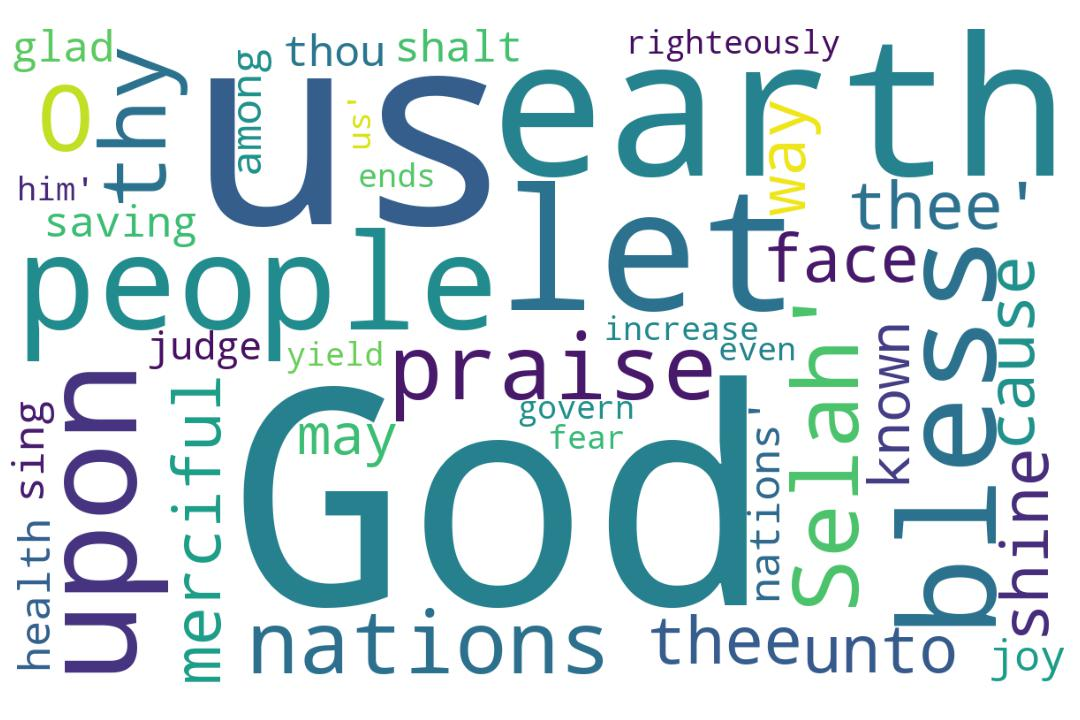
\includegraphics[width=\linewidth]{19OT-Psalms/Psalm67-WordCloud.jpg}
  \caption{Psalm 67 Word Cloud}
  \label{fig:Psalm 67 word Cloud}
\end{figure}


\marginpar{\scriptsize \centering \fcolorbox{bone}{lime}{\textbf{A PLEA FOR MERCY}}\\ (Psalm 67:1-7) \begin{compactenum}[I.][8]
    \item The \textbf{Cause of Comfort} \index[scripture]{Psalms!Psa 067:01}(Psa 67:1)
    \item A \textbf{Corporate Concern} \index[scripture]{Psalms!Psa 067:02}(Psa 67:2)
    \item A \textbf{Common Chorus} \index[scripture]{Psalms!Psa 067:04}(Psa 67:4)
    \item A \textbf{Cure for the Curse} \index[scripture]{Psalms!Psa 067:06}(Psa 67:6)
    \item A \textbf{Comforting Conclusion} \index[scripture]{Psalms!Psa 067:07}(Psa 67:7)
\end{compactenum}}

\footnote{\textcolor[rgb]{0.00,0.25,0.00}{\hyperlink{TOC}{Return to end of Table of Contents.}}}\footnote{\href{https://audiobible.com/bible/psalms_67.html}{\textcolor[cmyk]{0.99998,1,0,0}{Psalm 67 Audio}}}\textcolor[cmyk]{0.99998,1,0,0}{To the chief Musician on Neginoth, A Psalm \emph{or} Song.}\\
\\
\P  \textcolor[cmyk]{0.99998,1,0,0}{God be merciful unto us, and bless us; \emph{and} cause \fcolorbox{bone}{lime}{his face to shine} upon us; Selah.}\footnote{\textbf{Numbers 6:22-27} - And the LORD spake unto Moses, saying, [23] Speak unto Aaron and unto his sons, saying, On this wise ye shall bless the children of Israel, saying unto them, [24] The LORD bless thee, and keep thee: [25] The LORD make his face shine upon thee, and be gracious unto thee: [26] The LORD lift up his countenance upon thee, and give thee peace. [27] And they shall put my name upon the children of Israel; and I will bless them.}%\footnote{The key word to orient the reader shows up twice in seven verses (``Selah'' in verses 1 and 4). By now you know what the ``majority of conservative scholars'' are going to do with it. The entire Psalm deals with the Millennium and the Millennial Reign of the Son of God (see Psalm 2, 110; Isaiah 2, 11, etc.). ``God be merciful unto us and bless us...upon us.'' Verse 1 is a prayer for the restoration of Israel. Note especially the mid-Tribulation (or end-Tribulation) appearance of the Lord from heaven, as in the case of Job (Job 38:1), Saul (Acts 9:4--7), Daniel (Daniel 10:5--11), and Ezekiel (Ezekiel 1:1--4). We have commented on this under Psalm 31:16, which Kroll, Motyer, Yates, Jamieson, Baethgen, Briggs, Ewald, Dummelow, and Hengstenberg went by like they were in the Indianapolis 500. ``Thy saving health'' (vs. 2) is literal (see Psalm 91:3) and extends into eternity for the ``nations'' (see Revelation 22:2). ``All the people praise'' Him (see Psalm 2 and 110), and the ``nations'' will be glad and sing for joy, for the ``fulness of Israel'' (Romans 11:12) will affect nature (see Romans 8:20--27; Isaiah 11:1--10; Amos 9:13, etc.). The characteristics of the Millennium are Joy (vs. 4), Gladness (vs. 4), Blessing (vss. 1--7), Singing (vs. 4), Mercy (vs. 1), Praise (vs. 3), Righteousness (vs. 4), and Increase (vs. 6). This is the “Golden Age” of the unsaved philosophers; the “Thousand Year Reich” of the Nazis; the “Camelot” of the depraved Kennedy family; the “Great Society” of Lyndon Johnson, and the infamous “bringing in of Thy Kingdom” the Southern Baptists wasted their time on. It is the “Our Father” of the pagan Catholics answered at last—“thy kingdom come”— after those depraved killers had been praying it for sixteen hundred years. It came about without their help and despite their efforts, and when it came it destroyed their church, their theology, their priests and nuns, bishops and cardinals, archbishops and popes in one lick, because it was a Jewish kingdom (Luke 1:32). “Salvation is of the Jews” (John 4:22). Rome was never given the privilege, at either Advent, of saving anyone. \cite{Ruckman1992Psalms} }
[2] \textcolor[cmyk]{0.99998,1,0,0}{That thy way may be known upon earth, thy saving health \fcolorbox{bone}{lime}{among all nations}.} %\footnote{Ready for chaos? Here it is: ``May the people praise you...for you rule [present tense] the people justly'' (verses 3--4). This is the aborted perversion known as the New International Version. It simply erased the Millennial references. The nation’s knowledge of God is not even conditioned on God blessing Israel in the NIV, for the words “That thy way may be known” (vs. 2) have been removed from it. This is the godless abomination that bragged about how much more “readable” it was than the King James Bible and proved it by testing it out with a couple of hundred dead orthodox apostate kiddy school readers attached to dead orthodox churches. Not even the RSV of the NCC was this corrupt, although The Living Bible was; it did the same thing in order to disconnect the knowledge of God by the nations with the coming of the Lord. The Living Bible even destroys the sense of verse 1 by making it a present tense: ``as you look down on us.'' Kyle Yates (RSV committee) tells us that the Psalm is “Remarkable for its beauty, its simplicity and its world outlook.” (Can’t you guess what he is going to do? You get one guess!) “God’s gracious dealings are viewed as the means by which all people are led to turn to God...this is a striking universalistic note...expressing hope for God’s continued blessing in order that Israel’s mission may be completed.” \cite{Ruckman1992Psalms}} 
[3] \textcolor[cmyk]{0.99998,1,0,0}{Let the people praise thee, O God; let all the people praise thee.}
[4] \textcolor[cmyk]{0.99998,1,0,0}{O let the nations be glad and \fcolorbox{bone}{lime}{sing for joy}: for thou shalt judge the people righteously, and govern the nations upon earth. Selah.} %\footnote{Interpretation? “Rapunzel, Rapunzel, let down your golden hair.” No Advent, no return of Christ, no throne at Jerusalem, no Jesus Christ, no scriptural fulfillment, no restoration of Israel: just one big, godless, hellish, damnable denial of the main theme of the Bible, laden with enough piety and “godliness” to “gag a maggot” (circa 1980, Middle Schools). Kroll, being Premillennial, is finally forced to show his hand at verse 4, but not till then. He disassociates verse 1 from the Tribulation and the Advent and does away with the “saving health” by saying contemptuously it is “to be understood in the singular sense as salvation among all nations.” He didn’t make any connection with “health” at all, as it was given in Psalm 91:3; Ezekiel chapter 47; and Revelation 22:2; he equated “health” with Church Age salvation. Poor old Dummelow splashes around like a crippled thrasher in a bird bath. He wants the RV reading of Westcott and Hort put back into verses 4 and 6 and says that “God’s goodness to Israel reveals him [present tense] to the nations,” which of course is more nonsense. But Jamieson and Brown have the best way of saying what you don’t mean so you will think they mean what they think they didn’t say: “The manifest blessedness of Israel IN HER LORD shall attract all nations to the same Saviour...when all the people praise God then the earth itself shall be delivered from the curse...the future is to the eye of inspiration as sure as the already past...God’s blessing on the literal and spiritual Israel shall be the FORERUNNER of the conversion of the world.” Beautiful, ain’t it? No date given, no Lord returning, no Lord landing, no Lord reigning, no judgment on the nations, no judging the nations literally on earth, and no renovation of nature because of the King’s presence. The “blessing” came from people praising God. Dale Carnegie, Chuck Swindoll, Robert Schuller, and Norman Vincent Peale never did it any better. This is a typical masterpiece of “toning down,” “leavening,” and “stripping” a passage of its Biblical content. It is a dehydrating, blood letting, artificial preservative type of exposition that fills the works of the “godly scholars.” In the raw it is simply two things: unbelief and cowardice. \cite{Ruckman1992Psalms} }
[5] \textcolor[cmyk]{0.99998,1,0,0}{Let the people praise thee, O God; let all the people praise thee.}
[6] \textcolor[cmyk]{0.99998,1,0,0}{\emph{Then} shall the earth yield her increase; \emph{and} God, \emph{even} our own God, \fcolorbox{bone}{lime}{shall bless us}.}
[7] \textcolor[cmyk]{0.99998,1,0,0}{God shall bless us; and all the \fcolorbox{bone}{lime}{ends of the earth} shall fear him.}

\chapter{Proverb 8}

\begin{figure}
  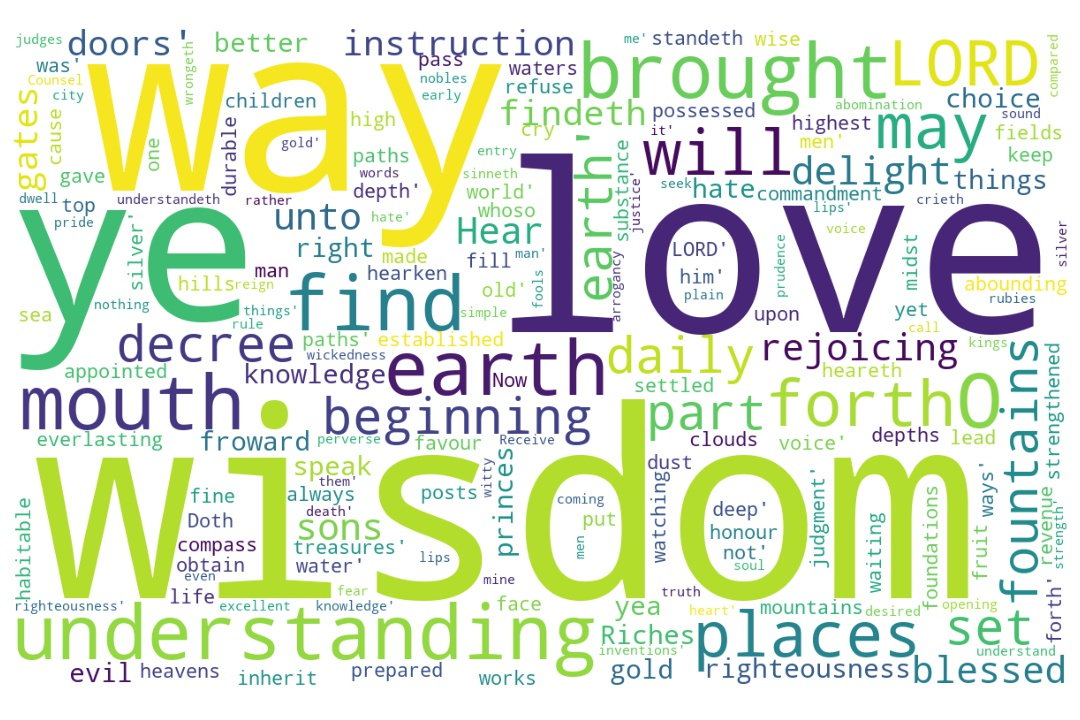
\includegraphics[width=\linewidth]{20OT-Proverbs/Proverb8-WordCloud.jpg}
  \caption{Proverb 8 Word Cloud}
  \label{fig:Proverb 8 Word Cloud}
\end{figure}

\marginpar{\scriptsize \centering \fcolorbox{bone}{lime}{\textbf{WHAT WISDOM DOES}}\\ (Proverb 8:1-36) \begin{compactenum}[I.][8]
    \item It \textbf{Cries}  \index[scripture]{Proverbs!Pro 08:01}(Pro 8:1)
    \item It \textbf{Calls}  \index[scripture]{Proverbs!Pro 08:04}(Pro 8:4)
    \item It is \textbf{Incomparable}  \index[scripture]{Proverbs!Pro 08:11}(Pro 8:11)
    \item It \textbf{Provides Counsel} \index[scripture]{Proverbs!Pro 08:14}(Pro 8:14)
    \item It \textbf{Offers Communion} \index[scripture]{Proverbs!Pro 08:17}(Pro 8:17)
    \item It \textbf{Causes} Success \index[scripture]{Proverbs!Pro 08:21}(Pro 8:21)
    \item It \textbf{Condemns} \index[scripture]{Proverbs!Pro 08:36}(Pro 8:36)\end{compactenum}}
    
\marginpar{\scriptsize \centering \fcolorbox{bone}{yellow}{\textbf{WISDOM IS THERE}}\\ (Proverb 8:1-36) \begin{compactenum}[I.][8]    \item There at the \textbf{Beginning} \index[scripture]{Proverbs!Pro 08}(Pro 8)
    \item There for a \textbf{Blessing} \index[scripture]{Proverbs!Pro 08}(Pro 8)
    \item There as a \textbf{Barrier} \index[scripture]{Proverbs!Pro 08}(Pro 8)
    \item There as a \textbf{Banner} \index[scripture]{Proverbs!Pro 08}(Pro 8)
    \item There to \textbf{Behold} \index[scripture]{Proverbs!Pro 08}(Pro 8)
    \item There in \textbf{Boldness} \index[scripture]{Proverbs!Pro 08}(Pro 8)
    \item There to \textbf{Abide} \index[scripture]{Proverbs!Pro 08}(Pro 8)
\end{compactenum}}    
    
\marginpar{\scriptsize \centering \fcolorbox{bone}{black}{\textbf{\textcolor[cmyk]{0,0,0,0}{MORE ABOUT WISDOM}}}\\ (Proverb 8:1-36) \begin{compactenum}[I.][8] 
      \item The \textbf{Message of Wisdom}  \index[scripture]{Proverbs!Pro 08:05} (Pro 8:5) 
    \item The \textbf{Majesty of Wisdom}  \index[scripture]{Proverbs!Pro 08:06} (Pro 8:6) 
    \item The \textbf{Manner of Wisdom}  \index[scripture]{Proverbs!Pro 08:06} (Pro 8:6) 
    \item The \textbf{Mouth of Wisdom}  \index[scripture]{Proverbs!Pro 08:07,08} (Pro 8:7, 8) 
    \item The \textbf{Mastery of Wisdom}  \index[scripture]{Proverbs!Pro 08:22-31} (Pro 8:22-31)
    \item The \textbf{Manna of Wisdom}  \index[scripture]{Proverbs!Pro 08:30} (Pro 8:30) 
    \item The \textbf{Man of Wisdom}  \index[scripture]{Proverbs!Pro 08:34} (Pro 8:34) 
\end{compactenum} }
  
\marginpar{\scriptsize \centering \fcolorbox{black}{blue}{\textbf{\textcolor[cmyk]{0,0,0,0}{WISDOM, CRYING OUT}}}\\ (Proverb 8:1-10) \begin{compactenum}[I.][8] 
     \item A \textbf{Pronounced} Cry \index[scripture]{Proverbs!Pro 08:01} (Pro 8:1) \footnote{Outlines inspired by Hubbard's \emph{The Preacher's Commentary - Proverbs} \cite{hubbard2004preacher}}
     \item A \textbf{Public} Cry \index[scripture]{Proverbs!Pro 08:02-03} (Pro 8:2-3) 
     \item A \textbf{Personal} Cry \index[scripture]{Proverbs!Pro 08:04-05} (Pro 8:4-5) 
     \item A \textbf{Proven} Cry \index[scripture]{Proverbs!Pro 08:06-09} (Pro 8:6-9) 
     \item A \textbf{Plain} Cry \index[scripture]{Proverbs!Pro 08:09} (Pro 8:9) 
     \item A \textbf{Purposeful} Cry \index[scripture]{Proverbs!Pro 08:09} (Pro 8:9) 
     \item A \textbf{Pointed} Cry \index[scripture]{Proverbs!Pro 08:10} (Pro 8:10
\end{compactenum} }

\marginpar{\scriptsize \centering \fcolorbox{bone}{orange}{\textbf{HE MINISTRY OF WISDOM}}\\ (Proverb 8:1-10) 
\begin{compactenum}[I.][8]     
    \item It \textbf{Gives Us Fear of the Lord}  \index[scripture]{Proverbs!Pro 08:13}(Pro 8:13)
    \item It \textbf{Grows Spectacular Fruit}  \index[scripture]{Proverbs!Pro 08:19}(Pro 8:19)
    \item It \textbf{Provides Fountains}  \index[scripture]{Proverbs!Pro 08:28}(Pro 8:28)
    \item It \textbf{Builds Foundations}  \index[scripture]{Proverbs!Pro 08:29}(Pro 8:29)
    \item It \textbf{Makes  a Way  to Get Favour from the Lord}  \index[scripture]{Proverbs!Pro 08:35}(Pro 8:35)
\end{compactenum} }
  
\footnote{\textcolor[cmyk]{0.99998,1,0,0}{\hyperlink{TOC}{Return to end of Table of Contents.}}}\footnote{\href{https://audiobible.com/bible/proverbs_8.html}{\textcolor[cmyk]{0.99998,1,0,0}{Proverbs Audio}}}\textcolor[cmyk]{0.99998,1,0,0}{Doth not wisdom \fcolorbox{bone}{lime}{cry}? and \fcolorbox{bone}{MYGOLD}{understanding} put forth her voice?}
[2] \textcolor[cmyk]{0.99998,1,0,0}{She standeth in the top of high places, by the way in the places of the paths.}
[3] \textcolor[cmyk]{0.99998,1,0,0}{She crieth at the gates, at the entry of the city, at the coming in at the doors.}
[4] \textcolor[cmyk]{0.99998,1,0,0}{Unto you, O men, I \fcolorbox{bone}{lime}{call}; and my voice \emph{is} to the sons of man.}
[5] \textcolor[cmyk]{0.99998,1,0,0}{O ye simple, understand wisdom: and, ye fools, be ye of an \fcolorbox{bone}{MYGOLD}{understanding} heart.}
[6] \textcolor[cmyk]{0.99998,1,0,0}{Hear; for I will speak of excellent things; and the opening of my lips \emph{shall} \emph{be} right things.}
[7] \textcolor[cmyk]{0.99998,1,0,0}{For my mouth shall speak truth; and wickedness \emph{is} an abomination to my lips.}
[8] \textcolor[cmyk]{0.99998,1,0,0}{All the words of my mouth \emph{are} in \fcolorbox{bone}{MYGOLD}{righteousness}; \emph{there} \emph{is} nothing froward or perverse in them.}
[9] \textcolor[cmyk]{0.99998,1,0,0}{They \emph{are} all plain to him that \fcolorbox{bone}{MYGOLD}{understandeth}, and right to them that find knowledge.}
[10] \textcolor[cmyk]{0.99998,1,0,0}{Receive my instruction, and not silver; and knowledge rather than choice gold.}
[11] \textcolor[cmyk]{0.99998,1,0,0}{For wisdom \emph{is} better than rubies; and all the things that may be desired are not to be \fcolorbox{bone}{lime}{compared} to it.}
[12] \textcolor[cmyk]{0.99998,1,0,0}{I wisdom dwell with prudence, and find out knowledge of witty inventions.}
[13] \textcolor[cmyk]{0.99998,1,0,0}{The fear of the LORD \emph{is} to hate evil: pride, and arrogancy, and the evil way, and the froward mouth, do I hate.}
[14] \textcolor[cmyk]{0.99998,1,0,0}{\fcolorbox{bone}{lime}{Counsel}emph{is} mine, and sound wisdom: I \emph{am} \fcolorbox{bone}{MYGOLD}{understanding}; I have strength.}
[15] \textcolor[cmyk]{0.99998,1,0,0}{By \fcolorbox{bone}{bone}{me} kings reign, and princes decree justice.}
[16] \textcolor[cmyk]{0.99998,1,0,0}{By \fcolorbox{bone}{bone}{me} princes rule, and nobles, \emph{even} all the judges of the earth.}
[17] \textcolor[cmyk]{0.99998,1,0,0}{I love them that love \fcolorbox{bone}{bone}{me}; and those that seek \fcolorbox{bone}{bone}{me} early \fcolorbox{bone}{lime}{shall find \fcolorbox{bone}{bone}{me}}.}
[18] \textcolor[cmyk]{0.99998,1,0,0}{Riches and honour \emph{are} with \fcolorbox{bone}{bone}{me}; \emph{yea}, durable riches and \fcolorbox{bone}{MYGOLD}{righteousness}.}
[19] \textcolor[cmyk]{0.99998,1,0,0}{My fruit \emph{is} better than gold, yea, than fine gold; and my revenue than choice silver.}
[20] \textcolor[cmyk]{0.99998,1,0,0}{I lead in the way of \fcolorbox{bone}{MYGOLD}{righteousness}, in the midst of the paths of judgment:}
[21] \textcolor[cmyk]{0.99998,1,0,0}{That I may \fcolorbox{bone}{lime}{cause} those that love \fcolorbox{bone}{bone}{me} to inherit substance; and I will fill their treasures.}
[22] \textcolor[cmyk]{0.99998,1,0,0}{The LORD possessed \fcolorbox{bone}{bone}{me} in the beginning of his way, before his works of old.}
[23] \textcolor[cmyk]{0.99998,1,0,0}{I was set up from everlasting, from the beginning, or ever the earth was.}
[24] \textcolor[cmyk]{0.99998,1,0,0}{When \emph{there} \emph{were} no depths, I was brought forth; when \emph{there} \emph{were} no fountains abounding with water.}
[25] \textcolor[cmyk]{0.99998,1,0,0}{Before the mountains were settled, before the hills was I brought forth:}
[26] \textcolor[cmyk]{0.99998,1,0,0}{While as yet he had not made the earth, nor the fields, nor the highest part of the dust of the world.}
[27] \textcolor[cmyk]{0.99998,1,0,0}{When he prepared the heavens, I \emph{was} there: when he set a compass upon the face of the depth:}\footnote{\textbf{Colossian 1:16-10} - For by him were all things created, that are in heaven, and that are in earth, visible and invisible, whether they be thrones, or dominions, or principalities, or powers: all things were created by him, and for him: [17] And he is before all things, and by him all things consist. [18] And he is the head of the body, the church: who is the beginning, the firstborn from the dead; that in all things he might have the preeminence. [19] For it pleased the Father that in him should all fulness dwell}.
[28] \textcolor[cmyk]{0.99998,1,0,0}{When he established the clouds above: when he strengthened the fountains of the deep:}\footnote{\textbf{Genesis 8:2} - The fountains also of the deep and the windows of heaven were stopped, and the rain from heaven was restrained;}\footnote{\textbf{Genesis 7:11} - In the six hundredth year of Noah’s life, in the second month, the seventeenth day of the month, the same day were all the fountains of the great deep broken up, and the windows of heaven were opened.}
[29] \textcolor[cmyk]{0.99998,1,0,0}{When he gave to the sea his decree, that the waters should not pass his commandment: when he appointed the foundations of the earth:}\footnote{\textbf{Genesis 1:6-8} - And God said, Let there be a firmament in the midst of the waters, and let it divide the waters from the waters. [7] And God made the firmament, and divided the waters which were under the firmament from the waters which were above the firmament: and it was so. [8] And God called the firmament Heaven. And the evening and the morning were the second day. }\footnote{\textbf{Job 38:4} - Where wast thou when I laid the foundations of the earth? declare, if thou hast understanding.}
[30] \textcolor[cmyk]{0.99998,1,0,0}{Then I was by him, \emph{as} one brought up \emph{with} \emph{him}: and I was daily \emph{his} delight, rejoicing always before him;}
[31] \textcolor[cmyk]{0.99998,1,0,0}{Rejoicing in the habitable part of his earth; and my delights \emph{were} with the sons of men.}
[32] \textcolor[cmyk]{0.99998,1,0,0}{Now therefore hearken unto \fcolorbox{bone}{bone}{me}, O ye children: for blessed \emph{are} \emph{they} \emph{that} keep my ways.}
[33] \textcolor[cmyk]{0.99998,1,0,0}{Hear instruction, and be wise, and refuse it not.}
[34] \textcolor[cmyk]{0.99998,1,0,0}{Blessed \emph{is} the man that heareth \fcolorbox{bone}{bone}{me}, watching daily at my gates, waiting at the posts of my doors.}
[35] \textcolor[cmyk]{0.99998,1,0,0}{For whoso findeth \fcolorbox{bone}{bone}{me} findeth life, and shall obtain favour of the LORD.}
[36] \textcolor[cmyk]{0.99998,1,0,0}{But he that sinneth against \fcolorbox{bone}{bone}{me} \fcolorbox{bone}{lime}{wrongeth his own soul}: all they that hate \fcolorbox{bone}{bone}{me} love death.}\footnote{\textbf{John 11:25} -  Jesus said unto her, \textcolor[cmyk]{0,0.85,0.70,0.23}{I am the resurrection, and the life: he that believeth in me, though he were dead, yet shall he live: 26 And whosoever liveth and believeth in me shall never die. Believest thou this?}}\footnote{\textbf{John 14:6} - Jesus saith unto him, \textcolor[cmyk]{0,0.85,0.70,0.23}{I am the way, the truth, and the life: no man cometh unto the Father, but by me.}}


% \textcolor[cmyk]{0,0.85,0.70,0.23}{




\end{document}

